\documentclass[10pt, a4paper]{article}
\title{\textbf{{\Huge 프리드버그 선형대수학 요약본}}}
\author{Lee Jhun Hyeok\,(wnsx0000@gmail.com)}
\date{\today}

\usepackage{graphicx} % Required for inserting images
\usepackage{kotex}
\usepackage{geometry}
\usepackage{parskip}
\usepackage{amsmath}
\usepackage{amsthm}

\usepackage{mdframed}
\newmdtheoremenv{DEF}{Definition}

\usepackage{tikz}
\usetikzlibrary{positioning}

\geometry{
 a4paper,
 left=25mm,
 right=25mm,
 top=30mm,
 bottom=30mm
 }
 \hbadness=199999  % or any number >=10000, 임시로 사용

\begin{document}
% 제목
\maketitle

% 목차
\textbf{\textit{목차}}

\textbf{\textit{Part 1. 벡터공간\\}}
1. 벡터공간\\
2. 부분공간\\
3. 일차결합과 연립일차방정식\\
4. 일차종속과 일차독립\\
5. 기저와 차원

\textbf{\textit{Part 2. 선형변환과 행렬\\}}
1. 선형변환\\
2. 선형변환의 행렬표현\\
3. 선형변환의 합성과 행렬 곱\\
4. 가역성과 동형사상\\
5. 좌표변환 행렬

\textbf{\textit{Part 3. 기본행렬연산과 연립일차방정식\\}}
1. 기본행렬연산과 기본행렬\\
2. 행렬의 랭크\\
3. 역행렬 구하기\\
4. 연립일차방정식 : 이론적 측면\\
5. 연립일차방정식 : 계산적 측면

\textbf{\textit{Part 4. 행렬식\\}}
1. 행렬식의 엄밀한 정의\\
2. n차 정사각행렬의 행렬식\\
3. 행렬식의 성질


\newpage


% 내용
%1.벡터공간
\part{\textit{\underline{벡터공간}}}

1장은 벡터공간에 대한 이야기임.

\part*{1. 벡터공간}

\section*{1. 벡터공간(vector space)}

\subsubsection*{1) 정의\\}
\begin{DEF}
체 $F$에서의 벡터공간(vector space) 또는 선형공간(linear space) $V$는 다음 8가지 조건을 만족시키는 두 연산, 합과 스칼라 곱을 가지는 집합임.

\begin{itemize}
\item 합(sum)은 $V$의 두 원소 $x, y$에 대하여 유일한 원소 $x+y \in V$를 대응하는 연산임.
\item 스칼라 곱(scalar multiplication)은 체 $F$의 원소 $a$와 벡터공간 $V$의 원소 $x$마다 유일한 원소 $ax \in V$를 대응하는 연산이다. 이때 $ax$는 $a$와 $x$의 스칼라 곱(product)이라 함.
\end{itemize}

(VS1) 모든 $x,y \in V$에 대하여 $x+y=y+x$임. (덧셈의 교환법칙)\\
(VS2) 모든 $x,y,z \in V$에 대하여 $(x+y)+z=x+(y+z)$임. (덧셈의 결합법칙)\\
(VS3) 모든 $x \in V$에 대하여 $x+0=x$인 $0 \in V$가 존재함. (덧셈에 대한 항등원, 즉 영벡터 존재)\\
(VS4) 각 $x \in V$마다 $x+y=0$인 $y \in V$가 존재함. (덧셈에 대한 역원, 즉 역벡터 존재)\\
(VS5) 각 $x \in V$에 대하여 $1x=x$임. (스칼라 곱에 대한 항등원 존재)\\
(VS6) 모든 $a,b \in F$와 모든 $x \in V$에 대하여 $(ab)x=a(bx)$임. (스칼라 곱에 대한 결합법칙)\\
(VS7) 모든 $a \in F$와 모든 $x,y \in V$에 대하여 $a(x+y)=ax+ay$임. (분배법칙)\\
(VS8) 모든 $a,b \in F$와 모든 $x \in V$에 대하여 $(a+b)x=ax+bx$임. (분배법칙)
\end{DEF}

\subsubsection*{2) 벡터공간의 표기}
체 $F$에서의 벡터공간 $V$는 $F-$벡터공간 $V$라고 표기함.

혼동의 여지가 없는 경우 체 $F$는 생략하기도 함.

\subsubsection*{3) 벡터와 스칼라}
벡터공간 $V$의 원소를 벡터, 체 $F$의 원소를 스칼라라 함.

여기서의 벡터는 벡터공간의 원소를 가리키는 일반적인 개념임.\\
지금까지 단순 화살표로 표현해 온 벡터를 포괄하는 의미.

(VS3)을 만족하는 유일한 벡터 $0$은 $V$의 영백터(zero vector)라 함.

(VS4)를 만족하는 유일한 벡터 $y$($-x$)는 덧셈에 대한 $x$의 역벡터(additive inverse)라고 함.


\newpage


\section*{2. 관련 정리}
\subsubsection*{1) 벡터 합의 소거법칙}
\textbf{Theorem 1.1}\, $x,y,z \in V$이고 $x+z=y+z$ 일 때, $x = y$ 임.

\textbf{Corollary 1}\, (VS3)을 만족하는 벡터 $0$(영백터)은 유일함.

\textbf{Corollary 2}\, (VS4)를 만족하는 벡터 $y$(역벡터)는 유일함.

\subsubsection*{2) 스칼라 곱 관련 성질\footnote{스칼라, 벡터, 영벡터 사이의 곱에 대한 정리.}}

\textbf{Theorem 1.2}\, 모든 벡터공간 $V$에 대해서 다음이 성립함.

\begin{enumerate}
    \item 모든 벡터 $x$에 대하여 $0x= \vec{0}$임.
    \item 모든 스칼라 $a$와 모든 벡터 $x$에 대하여 $(-a)x=-(ax)=a(-x)$임.
    \item 모든 스칼라 $a$에 대하여 $a \vec{0} = \vec{0}$임.\\
\end{enumerate}



\section*{3. 벡터공간의 예시\footnote{아래의 예시들은 각 성분별로(component-wise) 계산이 가능하기 때문에 매번 8가지 조건들을 검토할 필요가 없음.}}
\subsubsection*{1) $n$순서쌍(n-tuple)의 집합($F^n$)}
체 $F$에서 성분을 가져온 $n$순서쌍의 집합을 $F^n$이라 표기함.

$u=(a_1,a_2, ... ,a_n) \in F^n$, $v=(b_1,b_2, ... ,b_n) \in F^n$, $c \in F$ 일 때, 합과 스칼라 곱을 아래와 같이 정의하면 이 집합은 $F$-벡터공간임.

\[u+v=(a_1+b_1,a_2+b_2, ... ,a_n+b_n),\,cu=(ca_1,ca_2, ... ,ca_n)\]

$F^n$의 벡터는 행벡터(row vector)보다 열벡터(column vector)로 주로 표현함.

$F^1$은 그냥 $F$로 표현하는 경우가 많음.


\subsubsection*{2) 행렬(matrix)의 집합($M_{m \times n}(F)$)}
성분이 체 $F$의 원소인 모든 $m \times n$ 행렬의 집합은 $M_{m \times n}(F)$라 정의함.

$A,B \in M_{m \times n}(F)$, $c \in F$ 일 때, 합과 스칼라 곱을 아래와 같이 정의하면 이 집합은 $F$-벡터공간임.

\[(A+B)_{ij}=A_{ij}+B_{ij},\,(cA)_{ij}=cA_{ij}\]


\subsubsection*{3) 함수(function)의 집합($\mathcal{F}(S,F)$)}
체 $F$의 공집합이 아닌 부분집합 $S$가 있을 때, $\mathcal{F}(S,F)$는 $S$에서 $F$로 가는 모든 함수의 집합임.

$\mathcal{F}(S,F)$에서 모든 $s \in S$에 대하여 $f(s)=g(s)$일 때, 두 함수 $f$, $g$는 같다고 함.

$f,g \in \mathcal{F}(S,F)$, $c \in F$, $s \in S$ 일 때, 합과 스칼라 곱을 아래와 같이 정의하면 이 집합은 $F$-벡터공간임.

\[(f+g)(s)=f(s)+g(s),\,(cf)(s)=c(f(s))\]

실수집합 $R$에서 $R$로 가는 모든 연속함수의 집합을 $C(R)$이라 함.\\


\subsubsection*{4) 다항식(polynominal)의 집합($P(F)$)}
체 $F$에서 계수를 가져온 모든 다항식의 집합을 $P(F)$라 함.

두 다항식의 합과 스칼라 곱을 아래와 같이 정의하면 이 집합은 $F$-벡터공간임.

\[f(x)+g(x)=(a_n+b_n)x_n+(a_{n-1}+b_{n-1})x^{n-1}+ \cdots +(a_1+b_1)x+(a_0+b_0)\]
\[cf(x)=ca_nx_n+ca_{n-1}x^{n-1}+ \cdots +ca_1x+ca_0\]

음이 아닌 정수 $n$에 대하여 $P_n(F)$는 $n$ 이하의 차수를 가진 다항식의 집합임.


\subsubsection*{5) 수열의 집합}
체 $F$에서 정의된 모든 수열의 집합을 $V$라 할 때, $t \in F$와 두 수열 $(a_n)$, $(b_n)$에 대해서 합과 스칼라 곱을 정의하면 이 집합은 $F$-벡터공간임.

\[(a_n)+(b_n)=(a_n+b_n),\,t(a_n)=(ta_n)\]\\


\newpage


\part*{2. 부분공간(subspace)}

\section*{1. 부분공간\footnote{부분공간은 벡터공간의 일부분을 살펴보기 위해 존재한다고 이해하자.}}
\subsubsection*{1) 정의\\}
\begin{DEF}
$F$-벡터공간 $V$의 부분집합 $W$가 $V$에서 정의한 합과 스칼라 곱을 가진 $F$-벡터공간일 때, $W$를 $V$의 부분공간이라 함.
\end{DEF}

즉, 벡터공간인 부모의 연산을 그대로 물려받은 벡터공간인 부분집합.

모든 벡터공간 $V$에 대하여 $V$와 $\{ 0 \}$은 $V$의 부분공간임.\\
특히 ${0}$는 점공간인 부분공간(zero subspace)이라고 함.

\subsubsection*{2) 부분공간 판별}
어떤 부분집합이 부분공간이기 위한 필요충분조건은 아래 4가지 성질을 만족하는 것임.\\
벡터공간의 8가지 조건을 생각해 보면 당연한 이야기.

\begin{enumerate}
    \item 모든 $x \in W$, $y \in W$에 대하여 $x+y \in W$임. ($W$는 합에 대하여 닫혀 있음)
    \item 모든 $c \in F$와 모든 $x \in W$에 대하여 $cx \in W$임. ($W$는 스칼라 곱에 대하여 닫혀 있음)
    \item $W$는 영벡터를 포함함. (영벡터 존재)
    \item $W$에 속한 모든 벡터 각각의 덧셈에 대한 역벡터는 $W$의 원소임. (역벡터 존재)
\end{enumerate}

Theorem 1.3에 따르면 $W$와 $V$의 영벡터는 반드시 같고, 4번 성질은 굳이 확인할 필요가 없음(항상 성립)\\


\section*{2. 관련 정리}
\subsubsection*{1) 부분공간 판별}
\textbf{Theorem 1.3}\, 벡터공간 $V$와 그 부분집합 $W$에 대하여, $W$가 $V$의 부분공간이기 위한 필요충분조건은 아래의 세 가지 조건을 만족하는 것임.

\begin{enumerate}
    \item $0 \in W$
    \item 모든 $x \in W$, $y \in W$에 대하여 $x+y \in W$
    \item 모든 $c \in F$와 모든 $x \in W$에 대하여 $cx \in W$
\end{enumerate}

\subsubsection*{2) 부분공간의 교집합}

\textbf{Theorem 1.4}\, 벡터공간 $V$의 부분공간들의 임의의 교집합은 $V$의 부분공간임.\\


\newpage


\part*{3. 일차결합과 연립일차방정식}

\section*{1. 일차결합(linear combination)}

\subsubsection*{1) 정의\\}
\begin{DEF}
벡터공간 $V$의 공집합이 아닌 부분집합 $S$가 있다고 하자. 유한개의 벡터 $u_1,u_2, \cdots ,u_n \in S$와 스칼라 $a_1,a_2, \cdots , a_n$에 대하여 아래를 만족하는 벡터 $v \in V$를 $S$의 일차결합이라 함.

\[v=a_1u_1+a_2u_2+ \cdots +a_nu_n\]

이때, $v$는 벡터 $u_1,u_2, \cdots , u_n$의 일차결합이라 하고, $a_1,a_2, \cdots , a_n$은 이 일차결합의 계수(coefficient)라고 함.
\end{DEF}

영벡터는 공집합이 아닌 모든 부분집합의 일차결합임.\\


\section*{2. 연립일차방정식}
\subsubsection*{1) 일차결합과 연립일차방정식}
어떤 벡터가 일차결합으로 표현될 수 있는지를 연립일차방정식의 해를 구해 알아낼 수 있음.

어떤 벡터가 일차결합으로 표현될 수 있는지는 연립일차방정식의 풀이와 관련이 있는데, 여기서는 방법만 살펴보고 자세한 이야기는 3장에서 함.

\subsubsection*{2) 연립일차방정식의 풀이}
아래의 세 가지 연산을 반복하여 연립일차방정식이 아래의 성질을 가지도록 하면 미지수를 다른 미지수에 대하여 쉽게 풀 수 있음.

\textbf{연산1} \,두 방정식의 위치를 바꿈.\\
\textbf{연산2} \,방정식에 0이 아닌 상수를 곱함.\\
\textbf{연산3} \,상수를 곱하여 얻은 방정식을 다른 방정식에 더함.

\textbf{성질1} \,각 방정식에서 처음으로 등장하는 0이 아닌 계수는 1임.\\(맨 앞은 계수가 1)\\
\textbf{성질2} \,어떤 미지수가 어떤 방정식에서 처음 등장하면 그 외의 다른 행에서는 등장하지 않음.\\(맨 앞 미지수는 위아래가 비어있음)\\
\textbf{성질3} \,처음 등장하는 미지수의 첨자는 다음 행으로 내려갈 때마다 반드시 증가함.\\(맨 앞 미지수 첨자는 내려갈수록 커짐)

연산 도중 $0=c$(c는 0이 아닌 스칼라) 형태의 식이 나오면 해당 연립방정식은 해가 없음을 의미함.\\


\newpage


\section*{3. 생성공간}

\subsubsection*{1) 정의\\}
\begin{DEF}
벡터공간 $V$의 공집합이 아닌 부분집합 $S$에 대해서, $S$의 벡터를 사용하여 만든 모든 일차결합의 집합을 $S$의 생성공간(span)이라 하고, $span(S)$라 표기함.
\end{DEF}

편의를 위해 $span(\emptyset)= \{ 0 \}$으로 정의함.

\subsubsection*{2) 생성}
벡터공간 $V$의 부분집합 $S$에 대햐어 $span(S)=V$이면 $S$는 $V$를 생성한다(generate, span)고 하고, $S$를 $V$의 생성집합이라고 함.

$S$의 벡터가 $V$를 생성한다고 하기도 함.

어떤 벡터가 벡터공간을 생성하는지 확인하려면, 생성되는 벡터를 미지수로 놓고 완전히 성립하는지 보면 됨.\\

\section*{4. 관련 정리}
\subsubsection*{1) 생성공간과 부분공간 사이의 관계}
\textbf{Theorem 1.5}\, 벡터공간 $V$의 임의의 부분집합 $S$의 생성공간은 $S$를 포함하는 $V$의 부분공간임. 또한 $S$를 포함하는 $V$의 부분공간은 반드시 $S$의 생성공간을 포함함.

즉, 벡터공간의 부분집합으로 만든 생성공간(span)은 부분공간임.\\
또한 부분공간의 부분집합으로 만든 생성공간(span)은 해당 부분공간에 포함됨.\\


\newpage


\part*{4. 일차종속과 일차독립}

\section*{1. 일차종속(linearly dependent)/일차독립(linearly independent)}

\subsubsection*{1) 정의\\}
\begin{DEF}
벡터공간 $V$의 부분집합 $S$에 대하여 $a_1u_1+a_2u_2+ \cdots +a_nu_n=0$을 만족시키는 유한계의 서로 다른 벡터 $u_1,u_2, \cdots ,u_n \in S$와 적어도 하나는 0이 아닌 스칼라 $a_1,a_2, \cdots ,a_n$이 존재하면 집합 $S$는 일차종속(linearly dependent)라 함. 이때, $S$의 벡터 또한 일차종속이라 함.

벡터공간 $V$의 부분집합 $S$가 일차종속이 아니면 일차독립(linearly independent)라 함. 이때. $S$의 벡터 또한 일차독립이라 함.
\end{DEF}

\subsubsection*{2) 영벡터의 자명한 표현}
임의의 벡터 $u_1,u_2, \cdots ,u_n$에 대하여 $a_1=a_2= \cdots =a_n=0$이면 $a_1u_1+a_2u_2+ \cdots +a_nu_n=0$임. 이를 $u_1,u_2, \cdots ,u_n$의 일차결합에 대한 영벡터의 자명한 표현(trivial representation of 0)이라 함.

즉, 일차결합에서 스칼라에 전부 0을 넣어 표현한 영벡터를 의미함.


\subsubsection*{3) 일차독립인 집합에 대한 명제}
일차독립인 집합에 대한 아래의 명제들은 모든 벡터공간에서 참임.

\begin{enumerate}
    \item 공집합은 일차독립임.
    \item 영이 아닌 벡터 하나로 이루어진 집합은 일차독립임.
    \item 어떤 집합이 일차독립이기 위한 필요충분조건은 영벡터를 주어진 집합에 대한 일차결합으로 표현하는 방법이 자명한 방법 뿐인 것임.
\end{enumerate}

즉, 3번 명제를 사용하여 유한집합이 일차독립인지 확인할 수 있음.


\subsubsection*{4) 일차종속/일차독립이 가지는 의미}
일차독립\\
= 영벡터를 자명한 표현으로만 나타낼 수 있음.\\ 
= 해당 집합의 모든 벡터가 다른 벡터들의 일차결합으로 표현되지 않음.


\subsubsection*{5) 일차종속/일차독립의 판정}
1. 어떤 벡터가 다른 벡터들의 일차결합으로 표현되는지 확인.

2. 영벡터가 자명한 표현으로만 나타내지는지 확인.\\
연립일차방정식을 풀어서 확인할 수 있음.\\
3장의 행간소사다리꼴(RREF)에 대한 해석을 활용하여 확인할 수 있음.


\newpage


\section*{2. 관련 정리}
\subsubsection*{1) 일차종속/일차독립과 집합관계}

\textbf{Theorem 1.6}\, $V$는 벡터공간이고 $S_1 \subseteq S_2 \subseteq V$일 때, $S_1$이 일차종속이면 $S_2$도 일차종속임.

\textbf{Corollary 1}\, $V$는 벡터공간이고 $S_1 \subseteq S_2 \subseteq V$일 때, $S_2$가 일차독립이면 $S_1$도 일차독립임.

\subsubsection*{2) 일차독립과 벡터의 유일한 표현}

\textbf{Theorem 1.7}\, 벡터공간 $V$과 일차독립인 $V$ 부분집합 $S$가 있음. $S$에 포함되지 않는 벡터 $v \in V$에 대하여, $S \cup \{v\}$가 일차종속이기 위한 필요충분조건은 $v \in span(S)$임.

즉, 일차독립인 집합 $S$의 원소들을 일차결합하여 만들 수 있는 벡터가 $S$에 추가된 집합은 일차종속임. 반대로, 일차결합하여 만들 수 없는 벡터가 추가되면 여전히 일차독립임.

\begin{proof}
$S \cup \{ v \}$가 일차종속이면 $u_1,u_2, \cdots ,u_n \in S$와 스칼라 $a_1,a_2, \cdots ,a_{n+1}$에 대해서 $a_1u_1+a_2u_2+ \cdots +a_nu_n+a_{n+1}v=0$, $a_{n+1} \not= 0$이 성립함. 정리하면 $v = - \frac{1}{a_{n+1}}(a_1u_1+a_2u_2+ \cdots +a_nu_n+a_{n+1}v=0)$이므로 $v \in span(S)$임.
\end{proof}

\begin{proof}
$v \in span(S)$이므로 $v = a_1u_1+a_2u_2+ \cdots +a_nu_n+a_{n+1}v=0$으로 표현할 수 있고, 정리하면 $a_1u_1+a_2u_2+ \cdots +a_nu_n+(-1)v=0$으로 자명적이지 않은 표현이 존재하므로 $S \cup \{ v \}$는 일차종속임.
\end{proof}


\newpage


\part*{5. 기저와 차원}

\section*{1. 기저(basis)}

\subsubsection*{1) 정의\\}
\begin{DEF}
벡터공간 $V$와 부분집합 $\beta$에 대해서, $\beta$가 일차독립이고 $V$를 생성하면 $\beta$를 $V$의 기저(basis)라 함. $\beta$가 $V$를 형성할 때, $\beta$의 벡터는 $V$의 기저를 형성함.
\end{DEF}

즉, $V$의 기저인 $\beta$는 $V$를 생성하고 일차독립임.

기저는 유한집합이 아닐 수 있음.\footnote{ex. 집합 $\{1,x,x^2, \cdots \}$은 $P(F)$의 기저임.}


\subsubsection*{2) 표준기저}
벡터공간 $F^n$의 벡터 $e_1=(1,0, \cdots ,0),\,e_2=(0,1, \cdots ,0), \cdots ,e_n=(0, \cdots ,1)$에 대하여, 집합 $\{e_1,e_2, \cdots ,e_n\}$은 $F^n$의 표준기저임.\\
여기서의 $e_n$은 임의로 잡은 기호가 아니라, 벡터공간 $F^n$의 표준기저를 일반적으로 나타내는 기호임.

집합 $\{1,x,x^2, \cdots ,x^n\}$은 벡터공간 $P_n(F)$의 표준기저임.

행렬 $E^{ij} \in M_{m \times n}(F)$는 $i$행 $j$열 성분만 1이고, 나머지 성분은 0인 행렬임. 이를 $M_{m \times n}(F)$의 표준기저로 사용하기도 함.\\


\section*{2. 차원(dimension)}
\subsubsection*{1) 정의\\}
\begin{DEF}
기저가 유한집합인 벡터공간을 유한차원(finite dimension)이라 하고, 유한차원이 아닌 벡터공간을 무한차원(infinite dimension)이라 함. $V$의 기저가 $n$개의 벡터로 이루어질 때, 유일한 자연수 $n$은 $V$의 차원(dimension)이고, $dim(V)$라 표기함.
\end{DEF}

대체정리의 Corollary 1에서 알 수 있듯이, 기저를 형성하는 벡터의 개수는 벡터공간 $V$의 본질적 성질임.

\subsubsection*{2) 예시}
벡터공간 $\{0\}$의 차원은 0임.\\
벡터공간 $F^n$의 차원은 $n$임.\\
벡터공간 $M_(m \times n)(F)$의 차원은 $mn$임.\\
벡터공간 $P_n(F)$의 차원은 $n+1$임.\\
벡터공간 $P(F)$는 무한차원임.


\section*{3. 관련 정리}
\subsubsection*{1) 부분집합이 기저가 되기 위한 필요충분조건}
\textbf{Theorem 1.8}\, 벡터공간 $V$의 부분집합 $\beta = \{u_1,u_2, \cdots ,u_n\}$가 $V$의 기저이기 위한 필요충분조건은, 임의의 벡터 $v \in V$를 $\beta$에 속한 벡터의 일차결합으로 나타낼 수 있고 그 표현이 유일한 것임.

즉, 기저 $\beta$는 유일한 일차결합으로 $V$의 벡터\footnote{$\beta$의 벡터가 아닌 $V$의 벡터인 것 유의.}를 표현할 수 있고, $\beta$의 유일한 일차결합으로 $V$의 벡터가 표현된다면 $\beta$는 기저인 것.


\newpage


\subsubsection*{2) 생성집합과 기저의 관계\footnote{아래의 증명 방식을 눈여겨보자. 특히 일차독립인 집합을 생성하고, 그 집합이 벡터공간을 생성하는지 확인하는 방식에 집중할 것.}}
\textbf{Theorem 1.9}\, 유한집합 $S$가 벡터공간 $V$를 생성하면, $S$의 부분집합 중 $V$의 (유한집합인) 기저가 존재함.

\begin{proof}
$S=\emptyset$ 또는 $S=\{0\}$인 경우, $V=\{0\}$임. $\emptyset$은 일차독립이므로, $S$의 부분집합이면서 $V$의 기저임.

$S$가 영벡터가 아닌 벡터 $u_1$을 가지고 있다고 가정하면, $\{u_1\}$은 일차독립인 $S$의 부분집합임. 집합 $\{u_1,u_2, \cdots ,u_k\}$가 일차독립이 되도록 $S$에서 순차적으로 $u_2, \cdots ,u_k$를 꺼내서 추가하는 것을 유한 번 반복함. 최종적으로 얻은 일차독립인 집합을 $\beta = \{u_1,u_2, \cdots ,u_k\}$라 함.

$S$에서 일차독립인 부분집합을 추출했으니, 이제 이 부분집합이 $V$를 생성하는지 확인해야 함.\\
(i) $\beta = S$인 경우. $S$는 일차독립이고 $V$를 생성하므로 $V$의 기저임.\\
(ii) $\beta$가 $S$의 일차독립인 진부분집합인 경우. $span(\beta)$는 $V$의 부분공간이고, $S$를 포함하는 $V$의 부분공간은 $span(S)$(즉, $V$.) 또한 포함하므로\footnote{정리 1.5}, $S \subseteq span(\beta)$인지 증명하면 $\beta$는 $V$를 생성한다고 할 수 있음.

$v \in S$에 대하여 $v \in \beta$이면 당연히 $v \in span(\beta)$임. $v \notin \beta$이면 $\beta \cap \{v\}$는 $\beta$의 구성 방식에 의해 일차종속임. $\beta \cap \{v\}$가 일차종속이므로 $v \in span(\beta)$임\footnote{정리 1.7}. 따라서 $S \subseteq span(\beta)$임.
\end{proof}

\subsubsection*{3) 대체정리(replacement theorem)\footnote{대체정리는 수학적 귀납법으로 증명하지만 그 내용은 정리하지 않음. 여기서는 Corollary 1에 집중하자.}}
\textbf{Theorem 1.10}\, $n$개의 벡터로 이루어진 집합 $G$가 벡터공간 $V$를 생성한다고 하자. $L$이 $m$개의 벡터로 이루어진 일차독립인 $V$의 부분집합이면, $m \leq n$임. 또한 다음 조건을 만족시키는 $H \subseteq G$가 존재함. $H$는 $n-m$개의 벡터로 이루어졌으며, $L \cup H$는 $V$를 생성함.

\textbf{Corollary 1}\, 벡터공간 $V$가 유한집합인 기저를 포함한다고 가정하면, $V$의 모든 기저는 유한집합이며 같은 개수의 벡터로 이루어져 있음.

\begin{proof}
$\beta$가 $n$개의 벡터로 이루어진 $V$의 기저이고, $\gamma$가 또 다른 $V$의 기저라고 하자. $\gamma$가 $n+1$개의 벡터로 이루어져 있다고 하면, $\gamma$는 일차독립이고 $\beta$는 $V$를 생성하므로 대체정리에 의해 $n+1 < n$이 성립해야 하는데 이는 모순임. 즉, $\gamma$가 $m$개의 벡터로 이루어져 있다면 $m \leq n$임. $\beta$와 $\gamma$를 바꾸어 똑같은 논리를 반복하면 $n \leq m$이므로 $m=n$임. 즉, $V$의 모든 기저는 같은 개수의 벡터로 이루어져 있음.
\end{proof}

\textbf{Corollary 2}\, $V$를 차원이 $n$인 벡터공간이라 하자.\\
(1) $V$의 유한 생성집합에는 반드시 $n$개 이상의 벡터가 있음. 또한 $n$개의 벡터로 이루어진 $V$의 생성집합은 $V$의 기저임.\\
(2) 일차독립이고 $n$개의 벡터로 이루어진 $V$의 부분집합은 $V$의 기저임.\\
(3) 집합 $L \subset V$가 일차독립이면 $L \subseteq \beta$인 기저 $\beta$가 존재함. 즉, 일차독립인 $V$의 부분집합을 확장시켜 기저를 만들 수 있음.

3번 정리를 Basis Extension Theorem이라고 함. 일차독립인 집합으로 원하는 기저를 생성할 수 있다는 의미.

3장에서 등장하는 행간소사다리꼴(RREF)의 해석을 사용하면 일차독립인 집합으로 기저를 실제로 생성할 수 있음.

정리하면, 유한차원 벡터공간 $V$에서 $dim(V)=n$이라 할 때, 일차독립인 부분집합은 벡터의 개수가 $n$보다 클 수 없고, $V$를 생성하는 부분집합은 $n$보다 작을 수 없음. 기저는 일차독립인 집합의 집합과 생성집합의 집합의 교집합으로, 그 크기가 $n$임.


\newpage


\subsubsection*{4) 부분공간의 차원}
\textbf{Theorem 1.11}\, 유한차원 벡터공간 $V$에 대하여 부분공간 $W$는 유한차원이고, $dim(W) \leq dim(V)$임. 특히, $dim(W) = dim(V)$이면 $V=W$임.

\begin{proof}
$dim(V)=n$이라 하자. $W=\{0\}$이면 $W$는 유한차원이고 $dim(W)=0 \leq n$임. $W \neq \{0\}$ 인 경우, $W$는 영벡터가 아닌 벡터 $x_1$을 가지고, $\{x_1\}$은 일차독립임. $\{x_1,x_2, \cdots x_k\}$이 일차독립이 되도록 $W$에서 $x_1,x_2, \cdots ,x_k$를 꺼내자. $V$의 일차독립인 부분집합은 $n$개 이상의 벡터를 가질 수 없으므로, 이 과정은 $k \leq n$인 범위 안에서 끝남. 이때, $\{x_1,x_2, \cdots x_k\}$는 일차독립이고 $W$에서 벡터를 더 추가하면 일차종속이 되고, 해당 벡터는 $span(\{x_1,x_2, \cdots x_k\})$의 원소임. 즉, $\{x_1,x_2, \cdots x_k\}$는 $W$의 기저이고, $dim(W)=k \leq n$임.

$dim(W)=n$이면, $W$의 기저는 $n$개의 벡터로 이루어지고 일차독립인 $V$의 부분집합임. 대체정리의 Corollary 2에 의해 이 집합은 $V$의 기저임. 즉, $W=V$임.
\end{proof}

\textbf{Corollary 1}\, 유한차원 벡터공간 $V$의 부분공간 $W$에 대해서, $W$의 임의의 기저를 확장하여 $V$의 기저를 얻을 수 있음.

\begin{proof}
$W$의 임의의 기저는 일차독립인 $V$의 부분집합이므로, 대체정리의 Corollary 2에 의해 이를 확장시켜 $V$의 기저를 만들 수 있음.
\end{proof}


\newpage


%2.선형변환과 행렬
\part{\textit{\underline{선형변환과 행렬}}}

2장에서는 처음부터 끝까지 선형변환이 곧 행렬이고 행렬이 곧 선형변환이라는 이야기를 함.

\part*{1. 선형변환}

\section*{1. 선형변환(linear transformation)}

벡터공간의 성질을 보존하는 함수.

\subsubsection*{1) 정의\\}
\begin{DEF}
$F$-벡터공간 $V$와 $W$가 있다고 하자. 모든 $x,y \in V,\,c \in F$에 대하여 아래의 두 조건을 만족하는 함수 $T:\,V \rightarrow W$를 $V$에서 $W$로 가는 선형변환(linear transformation) 또는 선형(linear), 선형사상(linear map)이라 함.

\begin{enumerate}
\item $T(x+y)=T(x)+T(y)$
\item $T(ax)=aT(x)$
\end{enumerate}
\end{DEF}

즉, 연산을 하고 보내나 보내고 연산을 하나 똑같다는 것.

\subsubsection*{2) 선형의 성질}
성질1. $T$가 선형이면 $T(0)=0$임.

성질2. $T$가 선형이기 위한 필요충분조건은 모든 $x,y \in V$, $c \in F$에 대해서 $T(cx+y)=cT(x)+T(y)$인 것임.

성질3. $T$가 선형이면 모든 $x,y \in V$에 대해서 $T(x-y)=T(x)-T(y)$임.

성질4. $T$가 선형이기 위한 필요충분조건은 모든 $x_1,x_2, \cdots ,x_n \in V$와 $a_1,a_2, \cdots ,a_n \in F$에 대해서 아래의 식을 만족하는 것임.

\[
T(\sum_{i=1}^{n}{a_i x_i})=\sum_{i=1}^{n}{a_i T(x_i)}
\]

어떤 함수가 선형인지 보일 때, 주로 성질2를 사용함.

\subsubsection*{3) 항등변환(identity transformation)과 영변환(zero transformation)}
항등변환 $I_V : V \rightarrow V$는 모든 $x \in V$에 대해서 $I_V(x)=x$라 정의되는 선형임. 간단히 $I$라 표기하기도 함.\\
영변환 $T_0 : V \rightarrow W$는 모든 $x \in V$에 대해서 $T_0(x)=0$이라 정의되는 선형임.

\subsubsection*{4) 선형연산자(linear operator)}
정의역과 공역이 같은 선형변환. 다시 말해, 벡터공간 $V$에서 자기 자신으로 가는 선형변환.

\subsubsection*{5) 선형의 예시}
대표적인 선형 기하 변환으로는 회전, 대칭, 사영(한 값을 0으로 만드는 것)이 있음.\\
행렬을 전치행렬로 변환하는 함수, 미분, 적분 등 또한 선형임.\\


\newpage


\section*{2. 영공간(null space, kernel)과 상공간(range, image)}

\subsubsection*{1) 정의\\}
\begin{DEF}
벡터공간 $V, W$와 선형변환 $T:\,V \rightarrow W$가 있다고 하자.

영공간(null space, kernel)은 $T(x)=0$인 $x \in V$를 원소로 가지는 집합임. $N(T)$로 표기함.\\$N(T)=\{x \in V\,|\,T(x)=0\}$임.

상공간(range, image)은 $T$의 함숫값을 원소로 가지는 $W$의 부분집합임. $R(T)$라 표기함.\\$R(T)=\{T(x)\,|\,x \in V\}$
\end{DEF}

\section*{3. nullity와 rank}
\subsubsection*{1) 정의\\}
\begin{DEF}
벡터공간 $V,W$와 선형변환 $T:\,V \rightarrow W$에 대해서 $N(T)$와 $R(T)$가 유한차원이라 가정하자.

\begin{itemize}
    \item $N(T)$의 차원을 nullity(영공간의 차원)라 하고, $nullity(T)$라 표기함.
    \item $R(T)$의 차원을 rank(랭크, 계수)라 하고, rank(T)라 표기함.
\end{itemize}
\end{DEF}

\section*{4. 관련 정리}
\subsubsection*{1) 영공간/상공간은 부분공간임}
\textbf{Theorem 2.1}\, 벡터공간 $V, W$와 선형변환 $T:\,V \rightarrow W$에 대하여 $N(T)$, $R(T)$는 각각 $V, W$의 부분공간임.

\begin{proof}
$T(0)=0$이므로 $0 \in N(T)$임. $x,y \in N(T)$, $c \in F$에 대해서, $T(x+y)=0$, $T(cx)=0$이므로 합과 스칼라 곱에 대해 닫혀 있음. 그러므로 $N(T)$는 $V$의 부분공간임.

$T(0)=0$이므로 $0 \in R(T)$임. $x,y \in N(T)$, $c \in F$에 대해서, $T(v)=x, T(w)=y$인 $v,w \in V$가 존재함. $T(v+w)=x+y$, $T(cv)=cx$이므로 합과 스칼라 곱에 대해서 닫혀 있음. 그러므로 $R(T)$는 $V$의 부분공간임.
\end{proof}

\subsubsection*{2) 선형변환의 상공간 생성 방법}
\textbf{Theorem 2.2}\, 벡터공간 $V, W$와 선형변환 $T:\,V \rightarrow W$, 그리고 $V$의 기저 $\beta = \{v_1,v_2, \cdots ,v_n\}$에 대해서 아래의 식이 성립함.

\[
R(T)=span(T(\beta))=span(\{T(v_1),T(v_2), \cdots ,T(v_n)\})
\]

즉, $V$의 기저를 보내서 span하면 전체가 생성됨.

\begin{proof}
모든 $T(\beta)$는 $W$의 부분집합이고 $R(T)$는 부분공간이므로, $span(T(\beta)) \subseteq R(T)임.$\footnote{정리 1.5}

$w \in R(T)$이면 $w=T(v)$인 $v \in V$가 존재함. $\beta$는 $V$의 기저이므로, 아래와 같이 쓸 수 있음.

\[
v= \sum_{i=1}^{n}{a_i v_i}\,(a_1,a_2, \cdots ,a_n \in F)
\]

$T$가 선형이므로, $w=T(v)=T(\sum_{i=1}^{n}{a_i v_i})=\sum_{i=1}^{n}{a_i T(v_i)} \in span(T(\beta))$임. 즉, $R(T) \subseteq span(T(\beta))$임.

$span(T(\beta)) \subseteq R(T)$이고 $R(T) \subseteq span(T(\beta))$이므로 $R(T) = span(T(\beta))$임.
\end{proof}


\newpage


\subsubsection*{3) 차원정리(dimension theorem)}
\textbf{Theorem 2.3}\, 벡터공간 $V,W$와 선형변환 $T:\,V \rightarrow W$에 대하여 $V$가 유한차원이면 아래의 식이 성립함.

\[
nullity(T)+rank(T)=dim(V)
\]

선형변환 $T$에 대해서, $V$의 기저 중 일부는 0으로 가고 나머지는 상공간으로 간다는 의미.

아래의 다이어그램은 벡터공간 $V,W$와 선형변환 $T:V \rightarrow W$에 대해서, dimension theorem에서 기저가 어떻게 이동하는지를 보여줌.

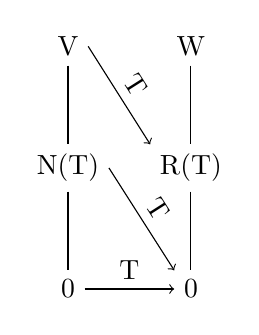
\begin{tikzpicture}
%Nodes
\node[]     (V)                     {V};
\node[]     (W)     [right=of V]    {W};
\node[]     (N)     [below=of V]    {N(T)};
\node[]     (R)     [below=of W]    {R(T)};
\node[]     (v0)    [below=of N]    {0};
\node[]     (w0)    [below=of R]    {0};

%Lines
\draw[-]    (V.south) -- (N.north);
\draw[-]    (W.south) -- (R.north);
\draw[->]   (V.east) -- (R.north west)
    node[midway, sloped, above]{T};
\draw[-]    (N.south) -- (v0.north);
\draw[-]    (R.south) -- (w0.north);
\draw[->]   (N.east) -- (w0.north west)
    node[midway, sloped, above]{T};
\draw[->]   (v0.east) -- (w0.west)
    node[midway, above]{T};
\end{tikzpicture}

\begin{proof}
차원정리의 증명은 4가지 단계로 이루어짐.

1. $kernel$의 기저 구성\\
$dim(V)=n$, $nullity(T)=k$라 하고, $N(T)$의 기저를 $\alpha = \{ v_1,v_2, \cdots v_k \}$라 하자.

2. $V$의 기저 구성\\
Theorem 1.11의 Corollary에 의해 $N(T)$의 기저를 확장하여 $V$의 기저를 만들 수 있음. $V$의 기저는 $\beta = \{ v_1,v_2, \cdots v_k,v_{k+1}, \cdots ,v_n \}$이라 하자.

3. 주장\\
$S=\{ T(v_{k+1}),T(v_{k+2}), \cdots ,T(v_n) \}$이 $R(T)$의 기저임을 보이면 증명이 완료됨.

4-1. 일차독립인지 확인\\
$a_1,a_2, \cdots ,a_n \in F$에 대해서 $\sum_{i=k+1}^{n}{a_{i}T(v_{i})}=0$이 성립한다고 하자. $\sum_{i=k+1}^{n}{a_{i}T(v_{i})}=T(\sum_{i=k+1}^{n}{a_{i}v_{i}})=0$이므로 $\sum_{i=k+1}^{n}{a_{i}v_{i}} \in N(T)$임. 즉, 이는 $N(T)$의 기저로 나타낼 수 있음. $b_1,b_2, \cdots ,b_n \in F$에 대해서 $\sum_{i=k+1}^{n}{a_{i}v_{i}}=\sum_{i=1}^{k}{b_{i}v_{i}}$, $-\sum_{i=1}^{k}{b_{i}v_{i}} + \sum_{i=k+1}^{n}{a_{i}v_{i}}=0$인데, $\beta$가 일차독립이므로 자명한 표현만이 성립함.

4-2. $R(T)$를 생성하는지 확인\\
상공간은 정의역 벡터공간의 기저를 보내서 확장하면 얻을 수 있고, $T(v_{1})=0,T(v_{2})=0, \cdots ,T(v_k)=0$임. 그러므로 $R(T)=span(T(\beta))=span(\{ T(v_{1}),T(v_{2}), \cdots ,T(v_n) \})=span(\{ T(v_{k+1}),T(v_{k+2}), \cdots ,T(v_n) \})=span(S)$임. 즉, $S$는 $R(T)$를 생성함.
\end{proof}

\subsubsection*{4) 단사함수의 확인}
\textbf{Theorem 2.4}\, 벡터공간 $V,W$와 선형변환 $T:\,V \rightarrow W$에 대해서, $T$가 단사함수이기 위한 필요충분조건은 $N(T)=\{0\}$인 것임.

\begin{proof}
$T$가 단사함수인 경우, $T(x)=0$인 $x$는 0밖에 없으므로 $N(T)=\{0\}$임.

$N(T)=\{0\}$인 경우, $T(x)=T(y)$라고 가정하자. $T(x)-T(y)=0$, $T(x-y)=0$인데 $N(T)=\{0\}$이므로 $x-y=0$, $x=y$임. 즉, $T$는 단사함수임.
\end{proof}


\newpage


\subsubsection*{5) 차원이 같은 경우 동치인 명제들}
\textbf{Theorem 2.5}\, 유한차원 벡터공간 $V,W$의 차원이 같을 때, 선형변환 $T:\,V \rightarrow W$에 대해서 아래의 세 명제는 동치임.

\begin{enumerate}
    \item $T$는 단사(one-to-one, injection)임.
    \item $T$는 전사(onto, surjection)임.
    \item $rank(T)=dim(V)$
\end{enumerate}

즉, 두 벡터공간의 차원이 같을 때 세 가지 명제 중 하나만 밝히면 나머지도 밝혀짐.

추가로, 이는 곧 해당 선형변환이 가역임을 의미함.

\begin{proof}
$T$가 단사임 $\Leftrightarrow$ $N(T)=\{0\}$ $\Leftrightarrow$ $nullity(T)=0$ $\Leftrightarrow$ $rank(T)=dim(V)=dim(W)$ $\Leftrightarrow$ $dim(R(T))=dim(W)$

$R(T)$는 $W$의 부분공간이므로 정리 1.11에 의해 차원이 같으면 $R(T)=W$임. 즉, $T$는 전사임.
\end{proof}


\subsubsection*{6) linear extension theorem}
\textbf{Theorem 2.6}\, $F$-벡터공간 $V,W$와 $V$의 기저 $\{v_1,v_2, \cdots ,v_n\}$을 생각하자. 벡터 $w_1,w_2, \cdots ,w_n \in W$에 대하여 아래의 조건을 만족시키는 선형변환 $T:\,V \rightarrow W$가 유일하게 존재함.\\

\begin{center}
$i=1,2, \cdots ,n$에 대하여 $T(v_i)=w_i$
\end{center}

즉, 정의역의 모든 값들을 보낼 필요 없이 기저의 원소만 보내 봐도 선형변환을 확정지을 수 있음. 기저에서 보낸 함숫값들의 조합은 선형변환에 따라 여러 가지가 있을 수 있는데, 각 조합에 대해서 선형변환이 유일하게 존재한다는 것.

선형변환을 정의하는 기본적인 방법. (기저만 보내면 충분함.)

선형변환의 행렬표현에서 기저만으로 선형변환을 정의하는 것은 linear extension theorem이 그래도 된다는 것을 보장하기 때문임.

\begin{proof}
$x \in V$는 $a_1,a_2, \cdots ,a_n \in F$에 대해서 $x=\sum_{i=1}^{n}{a_{i}v_{i}}$로 유일하게 표현할 수 있음.

선형변환 $T:\,V \rightarrow W$를 $T(v_i)=w_i$, $T(x)=\sum_{i=1}^{n}{a_{i}w_{i}}$라 정의하자.\footnote{이렇게 정의했을 때 해당 선형변환에 대해서 linear extension theorem이 성립하는지를 보는 것.}

(1) $T$는 선형인가?

$cT(v)+T(u)=T(cv+u)$가 성립함.

(2) $i=1,2, \cdots ,n$에 대하여 $T(v_i)=w_i$임.

(3) $T$는 유일한가?\footnote{정의한 $T(x)$가 유일한 선형변환임을 알 수 있음.}

선형변환 $U:\,V \rightarrow W$가 $i=1,2, \cdots ,n$에 대하여 $U(v_i)=w_i$를 만족한다고 가정하자. $x=\sum_{i=1}^{n}{a_{i}v_{i}} \in V$에 대해서, $U(x)=\sum_{i=1}^{n}{a_{i}w_{i}}=T(x)$이므로 $U=T$임.
\end{proof}

\textbf{Corollary}\, 두 벡터공간 $V,W$에 대하여 $V$가 유한집합인 기저 $\{v_1,v_2, \cdots ,v_n\}$를 포함한다고 가정하자. 두 선형변환 $U,T:\,V \rightarrow W$가 $i=1,2, \cdots ,n$일 때, $U(v_i)=T(v_i)$를 만족하면 $U=T$임.

즉, 기저에서 보낸 함숫값들의 조합이 같으면 같은 선형변환임.


\newpage


\part*{2. 선형변환의 행렬표현}

\section*{1. 순서기저(ordered basis)}

\subsubsection*{1) 정의\\}
\begin{DEF}
유한차원 벡터공간 $V$의 순서기저(ordered basis)는 순서가 주어진 기저임. 즉, 순서기저는 일차독립이며 $V$를 생성하는 벡터들로 이루어진 수열임.
\end{DEF}

같은 벡터로 이루어져 있더라도 순서가 다르면 다른 순서기저임.

\subsubsection*{2) 표준 순서기저(standard ordered basis)}
벡터공간 $F^n$의 표준 순서기저는 $\{e_1,e_2, \cdots ,e_n\}$임.\\
$P_n(F)$의 표준 순서기저는 $\{1,x, \cdots ,x_n\}$임.\\
$R^n$의 표준 순서기저는 $\{{(1,0, \cdots), \cdots ,(\cdots ,0,1,0, \cdots), \cdots ,(\cdots ,0,1)}\}$


\section*{2. 좌표벡터(coordinate vector)}

\subsubsection*{1) 정의\\}
\begin{DEF}
유한차원 벡터공간 $V$의 순서기저를 $\beta \{u_1,u_2, \cdots ,u_n\}$이라 하고, $x \in V$에 대해서 $a_1,a_2, \cdots ,a_n$은 $x = \sum_{i=1}^{n}{a_{i}u_{i}}$를 만족시키는 유일한 스칼라라 하자. $\beta$에 대한 좌표벡터(coordinate vector) $[x]_{\beta}$는 아래와 같음.

\[
[x]_{\beta} = 
\begin{pmatrix}
a_{1} \\
a_{2} \\
\vdots \\
a_{n}
\end{pmatrix}
\]
\end{DEF}

순서기저를 사용해 벡터를 $n$순서쌍으로 나타낸 것.\\
벡터를 좌표벡터로 표현하면 여러 계산에서 일종의 행렬로서 다룰 수 있게 됨.\\

\newpage


\section*{3. 선형변환의 행렬표현(matrix representation)}

선형변환을 행렬표현으로, 행렬표현을 선형변환으로 생각할 수 있음.

\subsubsection*{1) 정의\footnote{linear extension theorem이 이 정의가 가진 논리의 바탕이 됨.}\\}
\begin{DEF}
유한차원 벡터공간 $V,W$와 각각의 순서기저 $\beta = \{v_1, \cdots ,v_n\}$, $\gamma = \{w_1, \cdots ,w_m\}$, 선형변환 $T:\,V \rightarrow W$가 있음. $j=1,2, \cdots ,n$일 때, $j$마다 다음을 만족하는 유일한 스칼라 $a_{ij} \in F$가 존재함.

\[
T(v_{j})=\sum_{i=1}^{m}{a_{ij}w_i}
\]

성분이 $A_{ij}=a_{ij}$인 $m \times n$ 행렬 $A$를 순서기저 $\beta$, $\gamma$에 대한 선형변환 $T$의 행렬표현(matrix representation)이라 하고, $A=[T]_{\beta}^{\gamma}$라 표기함. $V=W$, $\beta=\gamma$이면 간단히 $A=[T]_{\beta}$라 표기함.
\end{DEF}

선형변환 $T:\,V \rightarrow W$에 대해서 $V$의 기저의 함숫값을 $W$의 기저로 나타낸 것.

$j$번째 열은 $\gamma$에 대한 $T(v_j)$의 좌표벡터라고 볼 수 있음.

linear extension theorem의 Corollary에 의해, 선형변환 $U:\,V \rightarrow W$가 $[U]_{\beta}^{\gamma}=[T]_{\beta}^{\gamma}$를 만족하면 $U=T$임.


\subsubsection*{2) 영변환의 행렬표현}
$T_{0}(v_j)=0=0w_1+0w_2+ \cdots +0w_m$이므로 $[T_{0}]_{\beta}^{\gamma}=O$($m \times n$영행렬)임.

즉, 영변환의 행렬표현은 영행렬임.

\subsubsection*{3) 항등변환의 행렬표현\footnote{항등변환은 그 정의상 정의역과 공역이 동일한 벡터공간임.}}
$I_{v_j}=v_j=0v_1+0v_2+ \cdots +1v_j+ \cdots +0v_n$이므로 $I_V$의 $j$열은 $e_j$이고, $[I_{V}]_{\beta}^{\beta}=[I_{V}]_{\beta}$는 아래와 같음.

\[
[I_{V}]_{\beta}^{\beta}=[I_{V}]_{\beta}=
\begin{pmatrix}
1 & 0 & \cdots & 0\\
0 & 1 & \cdots & 0\\
\vdots & \vdots & & \vdots\\
0 & 0 & \cdots & 1
\end{pmatrix}
\]

즉, 항등변환의 행렬표현은 $n \times n$ 항등행렬임.\\


\newpage


\section*{4. 선형변환의 집합 $\mathcal{L}(V,W)$\footnote{새로운 집합과 함수가 등장했으므로, 지금까지 배운 내용을 생각해 보면 $\mathcal{L}(V,W)$가 벡터공간인지, $U(T)=[T]_{\beta}^{\gamma}$가 선형변환인지는 당연히 생각해봐야 하는 주제임.}}

\subsubsection*{1) 정의\\}
\begin{DEF}
$F$-벡터공간 $V,W$에 대하여 $V$에서 $W$로 가는 모든 선형변환의 모임으로 이루어진 벡터공간을 $\mathcal{L}(V,W)$라 표기함. $V=W$이면 $\mathcal{L}(V,V)$를 간단히 $\mathcal{L}(V)$라 표기함.
\end{DEF}

Theorem 2.7에 의하면 $\mathcal{L}(V,W)$는 $F$-벡터공간임.

\subsubsection*{2) $[\cdot]_{\beta}^{\gamma}$는 선형변환인가?}
선형변환을 행렬표현으로 나타낼 수 있으므로, $T \in \mathcal{L}(V,W)$에 대해서 $U(T)=[T]_{\beta}^{\gamma}$인 $U:\mathcal{L}(V,W) \rightarrow M_{dim(W) \times dim(V)}(F)$라는 함수를 생각할 수 있음.

Theorem 2.8에 의하면 $U(T)=[T]_{\beta}^{\gamma}$는 선형변환임.

\subsubsection*{3) $\mathcal{L}(V,W)$의 기저}
$\mathcal{L}(V,W)$의 기저는 아래와 같음. (증명은 여종헌 프린트 참고.)

$$
T_{ij}(v_k)=\begin{cases}
    w_i\quad(k=j)\\
    0\,\,\quad(k \neq j)
\end{cases}
$$




\section*{5. 관련 정리}

\subsubsection*{1) $\mathcal{L}(V,W)$은 벡터공간인가?}
\textbf{Theorem 2.7}\, $F$-벡터공간 $V,W$와 선형변환 $T,U:V \rightarrow W$에 대하여 아래가 성립함.

먼저, 선형변환의 합과 스칼라 곱을 정의하자.\\
선형변환의 합과 스칼라 곱은 보편적인 함수의 집합($\mathcal{F}$)의 것과 같음.

\begin{enumerate}
    \item 임의의 $a \in F$에 대하여, $aT+U$는 선형임.
    \item 위 정의와 같이 선형변환의 합과 스칼라 곱을 정의할 때, $V$에서 $W$로 가는 모든 선형변환의 집합은 $F$-벡터공간임.
\end{enumerate}

선형변환의 집합($\mathcal{L}$)은 함수의 집합($\mathcal{F}$)의 부분공간임.

\begin{proof}
미리 정의한 함수의 합과 곱을 사용해 $(aT+U)(cx+y)=c(aT+U)(x)+(aT+U)(y)$임을 보이면 됨.

합과 곱에 대해서 닫혀 있고 $T_0$이 $\mathcal{L}(V,W)$에서 영벡터이므로 $\mathcal{L}(V,W)$는 벡터공간임.
\end{proof}


\subsubsection*{2) $U(T)=[T]_{\beta}^{\gamma}$는 선형변환인가?}
\textbf{Theorem 2.8}\, 유한집합 벡터공간 $V,W$와 각각의 순서기저 $\beta,\gamma$, 선형변환 $T,U:V \rightarrow W$에 대해서 아래가 성립함.

\begin{enumerate}
    \item $[T+U]_{\beta}^{\gamma}=[T]_{\beta}^{\gamma}+[U]_{\beta}^{\gamma}$
    \item 모든 스칼라 $a$에 대해서 $[aT]_{\beta}^{\gamma}=a[T]_{\beta}^{\gamma}$
\end{enumerate}

즉, $[\cdot]_{\beta}^{\gamma}$, 다시 말해 $U(T)=[T]_{\beta}^{\gamma}$는 선형변환임.

\begin{proof}
$\beta = \{v_1,v_2, \cdots ,v_n\}$, $\gamma = \{w_1,w_2, \cdots ,w_n\}$라 하자. $a_1, \cdots ,a_n, b_1, \cdots ,b_n \in F$, $j=1,2, \cdots ,n$에 대해서, $T(v_j)=\sum_{i=1}^{m}{a_{ij}w_i}$, $U(v_j)=\sum_{i=1}^{m}{b_{ij}w_i}$이고 $([T]_{\beta}^{\gamma})_{ij}=a_{ij}$, $([U]_{\beta}^{\gamma})_{ij}=b_{ij}$임. 이를 이용해 $(T+U)(v_j)$, $(aT)(v_j)$를 정리할 수 있음.
\end{proof}


\newpage


\part*{3. 선형변환의 합성과 행렬 곱}

\section*{1. 선형변환의 합성}

\subsubsection*{1) 새로운 연산의 필요성}
Theorem 2.9에 의하면 선형변환의 합성 또한 선형변환임.

지금까지 설명한 선형변환의 행렬표현은 선형변환의 합성에 대한 연산이 존재하지 않으므로 이를 정의해줘야 함.\\


\section*{2. 행렬 곱}

\subsubsection*{1) 정의\\}
\begin{DEF}
$m \times n$ 행렬 $A$와 $n \times p$ 행렬 $B$에 대하여 두 행렬 $A,B$의 곱(product) $AB$는 아래와 같이 정의된 $m \times p$ 행렬임.

\[
1 \leq i \leq m,\,1 \leq j \leq p,\,(AB)_{ij}= \sum^{n}_{k=1}A_{ik}B_kj
\]
\end{DEF}

이 행렬 곱은 두 선형변환의 합성을 행렬로서 나타낸 연산임.

\subsubsection*{2) 유도과정}
유한차원 벡터공간 $V,W,Z$와 선형변환 $T:V \rightarrow W$, $U:W \rightarrow Z$가 있음. $V$의 순서기저 $\{v_1, \cdots , v_n\}$, $W$의 순서기저 $\{w_1, \cdots , w_m\}$, $Z$의 순서기저 $\{z_1, \cdots , z_p\}$에 대하여 $A=[U]^{\gamma}_{\beta}$, $B=[T]^{\beta}_{\alpha}$라 하자.

$AB=[UT]^{\gamma}_{\alpha}$가 되도록 하는 행렬 곱을 정의할 것임. 선형변환의 행렬표현은 $T(v_{j})=\sum_{i=1}^{m}{a_{ij}w_i}$꼴에 의해 결정되므로, $(UT)(v_{j})$를 $\sum_{i=1}^{p}{C_{ij}z_i}$꼴로 나타내 $C_{ij}$에 대해 살펴볼 것임.

\begin{align*}
(UT)(v_j) &= U(T(v_j))=U(\sum_{k=1}^{m}{B_{kj}w_k})=\sum_{k=1}^{m}{B_{kj}}U(w_k)=\sum_{k=1}^{m}{B_{kj}}(\sum_{i=1}^{p}{A_{ik}z_i})=\sum_{i=1}^{p}{(\sum_{k=1}^{m}{A_{ik}B_{kj}})z_i}\\
&= \sum_{i=1}^{p}{C_{ij}z_i}\,(C_{ij}=\sum_{k=1}^{m}{A_{ik}B_{kj}})    
\end{align*}

즉, 성분이 $c_{ij}=C_{ij}$인 $q \times n$ 행렬 $c$는 선형변환 $UT$의 행렬표현 $[UT]_{\alpha}^{\gamma}$임.

여기서의 $C_{ij}=\sum_{k=1}^{m}{A_{ik}B_{kj}}$를 행렬 곱으로 정의함.

\subsubsection*{3) 행렬 곱과 행렬의 크기\footnote{이는 기저의 개수를 생각하면 당연함.}}
행렬 곱을 하는 두 행렬의 내부 차원이 같아야 행렬 곱이 정의됨.

행렬 곱을 하는 두 행렬의 외부 차원은 결과로 만들어지는 행렬의 크기를 결정함.

\subsubsection*{4) 연속적인 행렬 곱의 표현}
$n \times n$ 행렬 $A$에 대해서, $A^1=A,A^2=AA,A^3=A^2A, \cdots$로 정의함.
즉, 2 이상의 자연수 $k$에 대해서, $A^k=A^{k-1}A$라 정의함. 이때, $A^0=I_n$임.


\newpage


\section*{3. 선형변환의 합성과 행렬 곱 사이의 관계}
\subsubsection*{1) 대응관계}
행렬 곱의 유도과정과 Theorem 2.9에서 확인할 수 있듯이, 선형변환의 합성과 행렬 곱은 서로 완전히 대응됨.

\subsubsection*{2) 동일한 성질}
Theorem 2.10, 2.12, 2.16 등에서 확인할 수 있듯이, 선형변환의 합성과 행렬 곱은 아래의 성질들을 공유함.

\begin{enumerate}
    \item 분배법칙 성립.
    \item 결합법칙 성립.
    \item 항등원 존재. (항등변환, 항등행렬)
    \item 스칼라 곱의 분배법칙 성립.
    \item 교환법칙 성립하지 않음.\footnote{즉, $TU \neq UT$, $AB \neq BA$임}\\
    \item 곱셈의 소거법칙 성립하지 않음.
\end{enumerate}


\section*{4. 좌측 곱 변환}

행렬로 선형변환의 성질을, 또는 선형변환으로 행렬의 성질을 유추할 때 가장 유용하게 사용할 수 있는 도구.

\subsubsection*{1) 정의\\}
\begin{DEF}
$A$는 $m \times n$ 행렬이고, 성분은 체 $F$의 원소임. 아래의 선형변환을 간단히 $L_A$라 표기하자.

\[
L_A:F^n \rightarrow F^m,\, L_A(x)=Ax
\]

$L_A$를 좌측 곱 변환이라 함. 이때 $x$는 $F^n$의 열벡터이고, $Ax$는 $A$와 $x$의 행렬 곱임.
\end{DEF}

\subsubsection*{2) 성질}
Theorem 2.15에서 알 수 있듯이, 좌측 곱 변환은 선형이고 해당 Theorem에 서술한 여러 성질들을 가짐.

이 성질들을 이용해 행렬의 결합법칙을 증명할 수 있음.


\newpage


\section*{4. 관련 정리}

\subsubsection*{1) 선형변환의 합성은 선형변환인가?}
\textbf{Theorem 2.9}\, $F$-벡터공간 $V,W,Z$와 선형변환 $T:V \rightarrow W$, $U:W \rightarrow Z$를 생각하자. 두 선형변환의 합성 $UT:V \rightarrow Z$는 선형변환임.

\subsubsection*{2) 선형변환의 합성이 가지는 성질}
\textbf{Theorem 2.10}\, 벡터공간 $V$와 선형변환 $T,U_1,U_2 \in \mathcal{L}(V)$에 대해서 아래가 성립함.

\begin{enumerate}
    \item $T(U_1+U_2)=TU_1+TU_2$이고, $(U_1+U_2)T=U_1T+U_2T$ (분배법칙)
    \item $T(U_1U_2)=(TU_1)U_2$ (결합법칙\footnote{함수의 합성에서 결합법칙이 성립하는 것은 책의 부록에서 확인할 수 있음.})
    \item $TI=IT=T$
    \item 모든 스칼라 $a$에 대해서 $a(U_1U_2)=(aU_1)U_2=U_1(aU_2)$
\end{enumerate}

\subsubsection*{3) 선형변환의 합성과 행렬 곱}
\textbf{Theorem 2.11}\, 유한차원 벡터공간 $V,W,Z$와 각각의 순서기저 $\alpha,\beta,\gamma$, 선형변환 $T:V \rightarrow W$, $U:W \rightarrow Z$에 대해서 아래가 성립함.

\[
[UT]_{\alpha}^{\gamma}=[U]_{\beta}^{\gamma}[T]_{\alpha}^{\beta}
\]

행렬 곱의 유도과정과 정의를 생각하면 당연함.

\subsubsection*{4) 행렬 곱의 성질}
\textbf{Theorem 2.12}\, $A$가 $m \times n$ 행렬, $B$와 $C$가 $n \times p$ 행렬, $D$와 $E$가 $q \times m$ 행렬일 때, 다음이 성립함.

\begin{enumerate}
    \item $A(B+C)=AB+AC,\,(D+E)A=DA+EA$ (분배법칙)
    \item 임의의 스칼라 $a$에 대하여 $a(AB)=(aA)B=A(aB)$
    \item $I_{m}A=A=AI_{n}$
\end{enumerate}

이 성질은 각각 Theorem 2.10의 1, 4, 3과 대응됨.

\subsubsection*{5) 특정 열벡터 구하는 방법}
\textbf{Theorem 2.13}\, $m \times n$ 행렬 $A$와 $n \times p$ 행렬 $B$가 있음. $j=1,2, \cdots ,p$인 $j$에 대해서 $AB$의 $j$열을 $u_j$, $B$의 $j$열을 $v_j$라 표기하면 아래가 성립함.

\begin{enumerate}
    \item $u_j=Av_j$
    \item $v_j=Be_j$ (이때, $e_j$는 $F^p$의 $j$번째 표준 벡터\footnote{j번째만 1이고 나머지는 0인 tuple.})
\end{enumerate}

즉, AB의 특정 열벡터를 구하려면 A에다가 B의 (구하려는 순번의) 열벡터를 곱하면 됨.

B의 특정 열벡터를 구하려면 B 뒤에 $e_j$를 곱하면 됨.


\newpage


\subsubsection*{6) 좌표벡터의 행렬 곱}
\textbf{Theorem 2.14}\, $V,W$는 유한차원 벡터공간이고, 순서기저는 각각 $\beta, \gamma$임. 선형변환 $T:V \rightarrow W$와 $u \in V$에 대해서 아래가 성립함.

\[
[T(u)]_{\gamma}=[T]_{\beta}^{\gamma}[u]_{\beta}
\]

즉, 선형변환에 벡터를 대입하고 행렬로 표현하나, 선형변환의 행렬표현에 해당 벡터의 좌표벡터를 곱하나 동일함.

좌표벡터의 행렬 곱은 해당 선형변환에 대입하는 것과 같음.

\begin{proof}
$u \in V$를 고정하고 아래와 같은 선형변환 $f:F \rightarrow V,g:F \rightarrow W$를 정의하자.

\begin{center}
모든 $a \in F$에 대해서 $f(a)=au$, $g(a)=aT(u)$
\end{center}

$\alpha={1}$을 $F$의 표준 순서기저라 하자. $g =Tf$이므로 아래가 성립함.

\[
[T(u)]_{\gamma}=[g(1)]_{\gamma}=[g]_{\alpha}^{\gamma}=[Tf]_{\alpha}^{\gamma}=[T]_{\beta}^{\gamma}[f]_{\alpha}^{\beta}=[T]_{\beta}^{\gamma}[f(1)]_{\beta}=[T]_{\beta}^{\gamma}[u]_{\beta}
\]

\end{proof}

\subsubsection*{7) 좌측 곱 변환의 성질}
\textbf{Theorem 2.15}\, $A$는 $m \times n$ 행렬이고, 성분은 체 $F$의 원소임. 좌측 곱 변환 $L_A:F^n \rightarrow F^m$은 선형임.

또한 임의의 $m \times n$ 행렬 $B$(성분은 체 $F$의 원소)와 $F^n$의 표준 순서기저 $\beta$, $F^m$의 표준 순서기저 $\gamma$에 대해서 아래가 성립함.

\begin{enumerate}
    \item $[L_A]_{\beta}^{\gamma}=A$ (표준 순서기저에 대해서만 성립함.)
    \item $L_A=L_B \Longleftrightarrow A=B$
    \item $L_{A+B}=L_A+L_B$
    \item 모든 $a \in F$에 대하여 $L_{aA}=aL_A$
    \item $T:F^n \rightarrow F^m$가 선형이면 $T=L_C$가 되도록 하는 $m \times n$ 행렬 $C$가 유일하게 존재함. $C=[T]_{\beta}^{\gamma}$임.
    \item $L_{AE}=L_{A}L_{E}$ ($E$는 $n \times p$ 행렬)
    \item $m=n$이면 $L_{I_n}=I_{F^n}$임.
    \item $a_i$($1 \leq i \leq n$)가 $A$의 $i$번째 열일 때, $R(L_A)=span(\{a_1, \cdots ,a_n\})$임.
\end{enumerate}

\begin{proof}
    (1) $[L_A]_{\beta}^{\gamma}$의 $j$열은 $L_A(e_j)$와 같음. $L_A(e_j)=Ae_j$는 $A$의 $j$열이므로 $[L_A]_{\beta}^{\gamma}=A$임.
    
    (2) $A=[L_A]_{\beta}^{\gamma}=[L_B]_{\beta}^{\gamma}=B$
    
    (5) 모든 $x \in F^n$에 대해서 $T(x)=Cx=L_C(x)$이므로 $T=L_C$임. 2번 성질에 의해 $C$는 유일함.
\end{proof}

\subsubsection*{8) 행렬 곱의 결합법칙}
\textbf{Theorem 2.16}\, 행렬 곱에서 결합법칙이 성립함. 즉, $A(BC)$를 정의할 수 있는 행렬 $A,B,C$는 $(AB)C$도 정의할 수 있고 $A(BC)=(AB)C$임.

이는 Theorem 2.10의 2와 대응됨. (선형변환의 합성의 결합법칙 성립과 대응됨.)

\begin{proof}
$L_{A(BC)}=L_{A}L_{BC}=L_{A}(L_{B}L_{C})=(L_{A}L_{B})L_{C}=L_{AB}L_{C}=L_{(AB)C}$

Theorem 2.15의 2번 성질에 의해 $A(BC)=(AB)C$임.
\end{proof}


\newpage


\part*{4. 가역성과 동형사상}

\section*{1. 함수의 역함수(inverse)와 가역(invertible)}

\subsubsection*{1) 정의\\}
\begin{DEF}
벡터공간 $V,W$와 선형변환 $T:V \rightarrow W$를 생각하자. $TU=I_W$이고 $UT=I_V$인 함수 $U$를 $T$의 역함수(inverse)라 함. 이 역함수는 $T^{-1}$로 표기함. $T$가 가역이면 $T^{-1}$은 유일함.

역함수가 존재하는지를 가역(invertible)이라 함.
\end{DEF}

\subsubsection*{2) 성질/사실}
함수가 가역이기 위한 필요충분조건은 해당 함수가 단사(injection)이고 전사(subjection)인 것임.

$(TU)^{-1}=U^{-1}T^{-1}$ (사실1)

$(T^{-1})^{-1}=T$임. 특히, $T^{-1}$은 가역임. (사실2)

$V,W$가 차원이 같은 벡터공간일 때, 선형변환 $T:V \rightarrow W$가 가역일 필요충분조건은 $rank(T)=dim(V)$인 것임. (사실3)

\subsubsection*{3) 역함수(inverse)의 선형성}
Theorem 2.17에 의하면 선형변환의 역함수 또한 선형변환임.\\


\section*{2. 행렬의 역행렬(inverse)과 가역(invertible)}
\subsubsection*{1) 정의\\}
\begin{DEF}
$n \times n$ 행렬 $A$에 대해서 $AB=BA=I$인 $n \times n$ 행렬 $B$를 $A$의 역행렬(inverse)이라고 함. 이 역행렬은 $A^{-1}$로 표기함.

역행렬이 존재하는지를 가역(invertible)이라고 함.
\end{DEF}

정의에서 알 수 있듯이, 정사각행렬(정방행렬)이 아니면 가역일 수 없음.

행렬의 역행렬을 구하는 방법은 3절에서 다룸.

\subsubsection*{2) 성질}
$A$가 가역이면 $A$의 역행렬은 유일함.\\


\section*{3. 가역성의 판별}
\subsubsection*{1) 선형변환의 가역성 판별}
선형변환이 전단사인지를 확인함(Dimension Theorem, Theorem 2.4, Theorem 2.5). 또는 그 행렬표현이 가역인지를 확인함(Theorem 2.18).

\subsubsection*{2) 행렬의 가역성 판별}
$n \times n$ 행렬인 경우 랭크가 $n$인지 확인함. 또는 해당하는 선형변환이 가역인지를 확인함(Theorem 2.18).

행렬식이 0이 아닌지 확인함.


\newpage


\section*{4. 동형(isomorphic)과 동형사상(isomorphism)}
구체적으로는 다르지만 구조적으로는 같은 것을 동형(isomorphic)이라 함.

\subsubsection*{1) 정의\\}
\begin{DEF}
두 벡터공간 $V,W$ 사이에 가역인 선형변환 $T:V \rightarrow W$가 존재하면 $V$와 $W$는 동형(isomorphic)임. 이때 가역인 선형변환을 $V$에서 $W$로 가는 동형사상(isomorphism)이라 함.
\end{DEF}

무엇이 무엇과 동형이라는 개념은 동치관계임. 즉, $V$는 $V$와 동형이고, $V$가 $W$와 동형이면 $W$가 $V$와 동형이고, $V$가 $W$와 동형이고 $W$가 $S$와 동형이면 $V$가 $S$와 동형임.\\
간단히 정리하면 '그저 $V$와 $W$는 동형'인 것.

\subsubsection*{2) 동형이기 위한 필요충분조건}
Theorem 2.19에 의하면, 같은 체 위의 두 벡터공간의 차원이 같다면 두 벡터공간은 동형임.

즉, 차원이 같음 = 동형임 = 가역인 선형변환이 존재함.

\subsubsection*{3) 동형사상과 '이름 바꾸기'}
동형사상은 구조적으로 동일한 두 벡터공간을 이어준다는 점에서 벡터공간의 '이름만 바꾸는' 기능을 한다고 이해할 수 있음.

일례로, 선형변환의 행렬표현이 가능했던 것 또한 사실 선형변환의 집합과 행렬의 집합이 동형이고, $[]_{\beta}^{\gamma}$가 '선형변환의 이름을 행렬로 바꾸는' 동형사상이기 때문임.\\

아래의 그림은 벡터공간 $V,W$에 대해 동형사상(isomorphism) $T:V \rightarrow W$이 어떤 식으로 '이름을 바꾸는지'를 나타낸 다이어그램임. $V$의 연산을 $W$의 연산으로 바꾸고 있음.

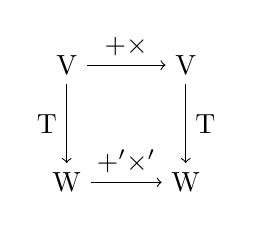
\begin{tikzpicture}
%Nodes
\node[]     (V1)                    {V};
\node[]     (V2)    [right=of V1]   {V};
\node[]     (W1)    [below=of V1]   {W};
\node[]     (W2)    [below=of V2]   {W};

%Lines
\draw[->]   (V1.east) -- (V2.west)
    node[midway, above]{$+ \times$};
\draw[->]   (W1.east) -- (W2.west)
    node[midway, above]{$+^{\prime} \times^{\prime}$};
\draw[->]   (V1.south) -- (W1.north)
    node[midway, left]{T};
\draw[->]   (V2.south) -- (W2.north)
    node[midway, right]{T};
\end{tikzpicture}


\section*{5. 표준표현(standard representation)}
\subsubsection*{1) 정의\\}
\begin{DEF}
체 $F$에서의 $n$차원 벡터공간 $V$의 순서기저를 $\beta$라 하자. $\beta$에 대한 $V$의 표준표현(standard representation)은 아래와 같이 정의된 함수 $\phi_{\beta}:V \rightarrow F^n$임.

\[
x \in V,\,\phi_{\beta}(x)=[x]_{\beta}
\]
\end{DEF}

즉, 벡터를 좌표벡터로 나타내는 함수.

\subsubsection*{2) 선형성과 동형성}
$\phi_{\beta}$는 선형변환임.

Theorem 2.21에 의하면 $\phi_{\beta}$는 벡터공간 $V$와 그 순서기저 $\beta$에 대해서 동형사상임.\\
이는 곧 $n$차원 벡터공간과 $F^n$이 동형이라는 것을 의미함.


\newpage


\subsubsection*{3) 선형변환 합성의 가환적 그래프}
차원이 각각 $n,m$인 벡터공간 $V,W$와 각각의 순서기저 $\beta, \gamma$, 선형변환 $T:V \rightarrow W$가 있다고 하자. $\phi_{\beta}$를 이용하면 $V$와 $F^n$을 동일시할 수 있고, $\phi_{\gamma}$를 이용하면 $W$와 $F^m$을 동일시할 수 있음. 즉, $T$와 $L_{[T]_{\beta}^{\gamma}}$또한 동일시할 수 있음. 이를 아래와 같이 수식으로 나타낼 수 있음.

\[
L_{[T]_{\beta}^{\gamma}}\phi_{\beta}=\phi_{\gamma}T
\]

이것을 이용하면 임의의 두 벡터공간 사이에 정의된 연산을 $F^n$과 $F^m$ 사이에 정의된 연산으로 나타낼 수 있음.

\begin{figure}[hbt!]
    \centering
    \includegraphics[width=5cm, height=5cm]{images/2.4.png}\\
\end{figure}

\section*{6. 관련 정리}
\subsubsection*{1) 역함수의 선형성}
\textbf{Theorem 2.17}\, 벡터공간 $V,W$와 가역인 선형변환 $T:V \rightarrow W$에 대해서 역함수 $T^{-1}:V \rightarrow W$ 또한 선형임.

\textbf{Corollary}\, 선형변환 $T:V \rightarrow W$가 가역이라고 하자. $V$가 유한차원이기 위한 필요충분조건은 $W$가 유한차원인 것임. 특히 이때 $dim(V)=dim(W)$임.

즉, 가역인 선형변환이 존재하면 두 벡터공간 모두가 유한차원이거나 무한차원이고, 유한차원인 경우 두 벡터공간의 차원도 같음.

\subsubsection*{2) 선형변환의 역함수와 행렬의 역행렬의 관계}
\textbf{Theorem 2.18}\, 유한차원 벡터공간 $V,W$와 각각의 순서기저 $\beta,\gamma$, 선형변환 $T:V \rightarrow W$에 대해서 $T$가 가역이기 위한 필요충분조건은 $[T]^{\gamma}_{\beta}$가 가역인 것임. 특히, $[T^{-1}]_{\gamma}^{\beta}=([T]_{\beta}^{\gamma})^{-1}$임.

이를 다이어그램으로 생각해 보면 이해가 편함.

\textbf{Corollary}\, $n \times n$ 행렬 $A$가 가역이기 위한 필요충분조건은 $L_A$가 가역인 것임. 특히, $(L_A)^{-1}=L_{A^{-1}}$임.

\subsubsection*{3) 동형이기 위한 필요충분조건}
\textbf{Theorem 2.19}\, 같은 체 위에서 정의된 유한차원 벡터공간 $V,W$에 대해서 $V$와 $W$가 동형이기 위한 필요충분조건은 $dim(V)=dim(W)$임.

\begin{proof}
1. $V,W$가 동형임. $\cdots$ $dim(V)=dim(W)$
$V,W$는 가역인 선형변환이 존재하고 유한차원이므로, Theorem 2.17의 Corollary에 의해 $dim(V)=dim(W)$임.

2. $dim(V)=dim(W)$ $\cdots$ $V,W$가 동형임.
$dim(V)=dim(W)=n$, $V$의 기저를 $\alpha=\{v_1, \cdots ,v_n\}$, $W$의 기저를 $\beta=\{w_1, \cdots ,w_n\}$라 하자. linear extension theorem에 의하면 $T(v_i)=w_i\,(1 \leq i \leq n)$인 선형변환 $T:V \rightarrow W$가 존재함. $R(T)=span(T(\alpha))=span(\beta)=W$이므로 $T$는 전사(onto, subjection)임. Theorem 2.5에 의해 $T$는 단사이므로 동형사상임.
\end{proof}


\newpage


\subsubsection*{4) $\Phi^{\gamma}_{\beta}$의 동형성}
\textbf{Theorem 2.20}\, 차원이 각각 $n,m$인 $F$-벡터공간 $V,W$를 생각하자. $V,W$의 순서기저를 각각 $\beta,\gamma$라 할 때, 아래와 같이 정의한 함수 $\Phi^{\gamma}_{\beta}:\mathcal{L}(V,W) \rightarrow M_{m \times n}(F)$는 동형사상임.

\[
T \in \mathcal{L}(V,W),\,\Phi^{\gamma}_{\beta}=[T]^{\gamma}_{\beta}
\]

즉, 선형변환의 집합과 행렬의 집합은 동형이고, 선형변환의 행렬표현을 나타내는 $[]_{\beta}^{\gamma}$, 즉 $\Phi^{\gamma}_{\beta}$는 동형사상임.\\
이를 Fundamental Theorem of Linear Algebra라고 함. (선형사상=행렬)

\begin{proof}
동형사상은 가역인 선형변환임. Theorem 2.8에 의하면 $\Phi^{\gamma}_{\beta}$는 선형이므로 전단사인 것을 보여야 함. 임의의 $m \times n$ 행렬 $A$에 대해서 $\Phi^{\gamma}_{\beta}(T)=A$인 선형변환 $T:V \rightarrow W$가 유일하게 존재함을 보이면 됨.

$\beta=\{v_1, \cdots ,c_n\}$, $\gamma=\{w_1, \cdots ,w_m\}$이라 하면, linear extension theorem에 의해 아래와 같이 정의된 선형변환 $T:V \rightarrow W$가 유일함.

\[
T(v_j)=\sum_{i=1}^{m}A_{ij}w_i\,(1 \leq j \leq n)
\]

즉, 행렬 $A$에 대해 선형변환 $T$가 유일함.

+ 여종헌 프린트에 $\mathcal{L}(V,W)$의 차원을 직접 구해 증명하는 방법도 나와있음.
\end{proof}

\textbf{Corollary}\, 차원이 각각 $n,m$인 유한차원 벡터공간 $V,W$에 대해서 $\mathcal{L}(V,W)$는 차원이 $nm$인 벡터공간임.

\subsubsection*{5) $\phi_{\beta}$의 동형성}
\textbf{Theorem 2.21}\, 임의의 유한차원 벡터공간 $V$와 순서기저 $\beta$에 대해서 $\phi_{\beta}$는 동형사상임.


\newpage

\part*{5. 좌표변환 행렬}

\section*{1. 좌표변환 행렬(change of coordinate matrix)}

\subsubsection*{1) 정의\\}
\begin{DEF}
Theorem 2.22에 의하면, 유한차원 벡터공간 $V$의 두 순서기저 $\beta, \beta^{\prime}$에 대해서, $Q=[I_V]^{\beta}_{\beta^{\prime}}$라 하자. 아래가 성립함.

\begin{enumerate}
    \item $Q$는 가역행렬임.
    \item 임의의 $v \in V$에 대해서 $[v]_{\beta}=Q[v]_{\beta^{\prime}}$
\end{enumerate}
\end{DEF}

즉, 좌표변환 행렬은 벡터공간의 어떤 벡터에 대해서, 특정 기저로 표현한 좌표벡터를 다른 기저로 표현한 좌표벡터로 만들 수 있는 것.

$Q$는 $\beta^{\prime}$좌표를 $\beta$좌표로 변환함.

이때, $Q^{-1}$은 $\beta$좌표를 $\beta^{\prime}$좌표로 변환함.\\


\section*{2. 선형변환 행렬표현의 전환}
\subsubsection*{1) 선형변환 행렬표현의 전환}
Theorem 2.23에 의하면, 한 선형변환의 행렬표현을 다른 기저를 이용한 동일한 선형변환의 행렬표현으로 전환할 수 있음. 아래가 그 식임. 이때 $Q$는 $\beta^{\prime}$좌표를 $\beta$좌표로 옮기는 좌표변환 행렬임.

\begin{center}
$[T]_{\beta^{\prime}}=[I_V]_{\beta}^{\beta^\prime}[T]^{\beta}_{\beta}[I_V]_{\beta^{\prime}}^{\beta}=Q^{-1}[T]_{\beta}Q$
\end{center}

\begin{center}
$[T]_{\beta}=[I_V]^{\beta}_{\beta^\prime}[T]^{\beta^{\prime}}_{\beta^{\prime}}[I_V]^{\beta^{\prime}}_{\beta}=Q[T]_{\beta^{\prime}}Q^{-1}$    
\end{center}

\begin{center}
$[T]_{\alpha}^{\beta}=[I_W]_{\beta^\prime}^{\beta}[T]_{\alpha^{\prime}}^{\beta^{\prime}}[I_V]_{\alpha}^{\alpha^{\prime}}$\\
\end{center}


\section*{3. 닮음(similar)\footnote{닮음에 대한 자세한 이야기는 5~7장에서 다룸.}}
\subsubsection*{1) 정의\\}
\begin{DEF}
$A,B$가 $M_{n \times n}(F)$의 행렬이라 하자. $B=Q^{-1}AQ$인 가역행렬 $Q$가 존재하면 $B$는 $A$와 서로 닮음(similar)임.
\end{DEF}

즉, 동일한 선형변환에 대해 서로 다른 두 행렬표현은 서로 닮음(similar)임.

닮음 관계는 동치관계임.

서로 닮은 행렬들에 대해서 모두 같은 값을 갖는 것들이 있음. 즉, invariant인 것들이 있음. invariant에는 랭크(rank), 행렬식(determinant), 대각합(trace) 등이 있음.\footnote{invariant에 속하는 것들은 뒷 장에서 계속해서 등장함.}


\newpage


\section*{4. 관련 정리}
\subsubsection*{1) 좌표변환 행렬(change of coordinate matrix)의 정의}
\textbf{Theorem 2.22}\, 유한차원 벡터공간 $V$의 두 순서기저 $\beta, \beta^{\prime}$에 대해서, $Q=[I_V]^{\beta}_{\beta^{\prime}}$라 하자. 아래가 성립함.

\begin{enumerate}
    \item $Q$는 가역행렬임.
    \item 임의의 $v \in V$에 대해서 $[v]_{\beta}=Q[v]_{\beta^{\prime}}$
\end{enumerate}

$Q$는 $\beta^{\prime}$좌표를 $\beta$좌표로 변환한다고 함.

\begin{proof}
1. $Q=[I_V]^{\beta}_{\beta^{\prime}}$인데, $I_V$가 가역이므로, $Q$ 또한 가역임.

2. $[v]_{\beta}=[I_V(v)]_{\beta}=[I_V]_{\beta^{\prime}}^{\beta}[v]_{\beta^{\prime}}=Q[v]_{\beta^{\prime}}$
\end{proof}

\subsubsection*{2) 선형변환 행렬표현의 전환}
\textbf{Theorem 2.23}\, 유한차원 벡터공간 $V$의 선형연산자 $T$와 $V$의 순서기저 $\beta$, $\beta^{\prime}$이 있음. $Q$가 $\beta^{\prime}$좌표를 $\beta$좌표로 옮기는 좌표변환 행렬이라 하면 아래가 성립함.

\[
[T]_{\beta^{\prime}}=[I_V]_{\beta}^{\beta^\prime}[T]^{\beta}_{\beta}[I_V]_{\beta^{\prime}}^{\beta}=Q^{-1}[T]_{\beta}Q
\]

즉, $T$가 유한차원 벡터공간 $V$의 선형연산자이고 $\beta$와 $\beta^{\prime}$이 $V$의 순서기저일 때, $[T]_{\beta^{\prime}}$과 $[T]_{\beta}$는 서로 닮음(similar)임.

이를 더 일반화하여 $V,W$ 사이에 정의된 선형변환 $T:V \rightarrow W$에 대해 나타내면 아래와 같음.

\[
[T]_{\alpha}^{\beta}=[I_W]_{\beta^\prime}^{\beta}[T]_{\alpha^{\prime}}^{\beta^{\prime}}[I_V]_{\alpha}^{\alpha^{\prime}}
\]

\begin{proof}
방법1. 선형변환 행렬표현의 전환을 함수의 합성으로 나타내기.

벡터공간 $V$의 기저 $\alpha, \alpha^{\prime}$와 $W$의 기저 $\beta, \beta^{\prime}$에 대해서, 벡터의 이동을 고려하면 아래의 다이어그램을 생각할 수 있음. 즉, $[T]_{\alpha}^{\beta}=[I_W]_{\beta^\prime}^{\beta}[T]_{\alpha^{\prime}}^{\beta^{\prime}}[I_V]_{\alpha}^{\alpha^{\prime}}$임. $W$ 대신 $V$를 넣으면 위 식을 유도할 수 있음.

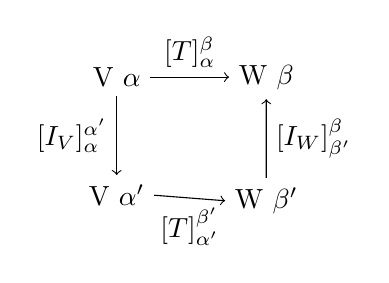
\begin{tikzpicture}[scale=10]
%Nodes
\node[]     (V1)                    {V $\alpha$};
\node[]     (V2)    [below=of V1]   {V $\alpha^{\prime}$};
\node[]     (W1)    [right=of V1]   {W $\beta$};
\node[]     (W2)    [below=of W1]   {W $\beta^{\prime}$};

%Lines
\draw[->]   (V1.south) -- (V2.north)
    node[midway, left]{$[I_V]_{\alpha}^{\alpha^{\prime}}$};

\draw[->]   (W2.north) -- (W1.south)
    node[midway, right]{$[I_W]_{\beta^{\prime}}^{\beta}$};

\draw[->]   (V1.east) -- (W1.west)
    node[midway, above]{$[T]_{\alpha}^{\beta}$};
    
\draw[->]   (V2.east) -- (W2.west)
    node[midway, below]{$[T]_{\alpha^{\prime}}^{\beta^{\prime}}$};
\end{tikzpicture}

방법2. 단순 유도하기.

$Q[T]_{\beta^{\prime}}=[I]_{\beta^{\prime}}^{\beta}[T]_{\beta^{\prime}}^{\beta^{\prime}}=[IT]_{\beta^{\prime}}^{\beta}=[TI]_{\beta^{\prime}}^{\beta}=[T]_{\beta}^{\beta}[I]_{\beta^{\prime}}^{\beta}=[T]_{\beta}Q$
\end{proof}

\textbf{Corollary}\, $A \in M_{n \times n}(F)$와 $F^n$의 순서기저 $\gamma$에 대해서 아래가 성립함.

\[
[L_A]_{\gamma}=Q^{-1}AQ
\]

이때, $n \times n$ 행렬 $Q$의 $j$열은 $\gamma$의 $j$번째 벡터임.


\newpage


%3.기본행렬연산과 연립일차방정식
\part{\textit{\underline{기본행렬연산과 연립일차방정식}}}
\part*{1. 기본행렬연산과 기본행렬}

\section*{1. 기본연산(elementary operation)}

\subsubsection*{1) 정의\\}
\begin{DEF}
$m \times n$ 행렬 $A$에 대해서 $A$의 행[열]에 대한 아래의 세 연산을 기본행[열]연산(elementary row[column] operation)이라 함.

\begin{enumerate}
    \item $A$의 두 행[열]을 교환하는 것.
    \item $A$의 한 행[열]에 영이 아닌 스칼라를 곱하는 것.
    \item $A$의 한 행[열]에 다른 행[열]의 스칼라 배를 더하는 것.
\end{enumerate}

행연산(row operation)과 열연산(column operation)을 통틀어 기본연산(elementary operation)이라 함.

기본연산의 1, 2, 3을 각각 1형(type), 2형, 3형이라 함.
\end{DEF}

\section*{2. 기본행렬(elementary matrix)}

\subsubsection*{1) 정의\\}
\begin{DEF}
$n \times n$ 기본행렬(elementary matrix)은 항등행렬 $I_n$에 기본연산을 한 번 적용하여 얻은 행렬임.

$I_n$에 1형, 2형, 3형 연산을 하여 얻은 행렬을 각각 1형, 2형, 3형이라고 함.
\end{DEF}

\subsubsection*{2) 기본연산의 적용}
Theorem 3.1에 의하면, 기본연산을 적용하는 것은 그 행렬에 적절한 기본행렬을 곱하는 것과 같음.

이 덕분에 기본연산을 적용하는 것을 수식적으로 나타낼 수 있음.


\section*{3. 관련 정리}
\subsubsection*{1) 기본연산과 기본행렬의 곱}
\textbf{Theorem 3.1}\, 행렬 $A \in M_{m \times n}(F)$에 기본행[열]연산을 하여 행렬 $B$를 얻었다면, $B=EA[B=AE]$가 되는 $m \times m[n \times n]$ 기본행렬 $E$가 존재함. 이때, $A$에서 $B$를 얻은 기본행[열]연산을 $I_m[I_n]$에 똑같이 적용하면 행렬 $E$가 됨. 역으로 $E$가 $m \times m[n \times n]$ 기본행렬일 때, $I_m[I_n]$에서 $E$를 얻은 기본행[열]연산을 $A$에 똑같이 적용하면 $EA[AE]$가 됨.

즉, 기본행렬을 곱하는 것은 그 기본행렬에 해당하는 기본연산을 적용하는 것과 같음.

\subsubsection*{2) 기본행렬의 가역성}
\textbf{Theorem 3.2}\, 기본행렬은 가역임. 그 역행렬은 같은 종류의 기본행렬임.

\begin{proof}
기본행렬을 만든 연산을 거꾸로 수행하면(해당하는 기본행렬 곱하면) 항등행렬이 나오므로 기본행렬은 가역임.\\
\end{proof}


\newpage


\part*{2. 행렬의 랭크}

행렬의 랭크로 임의의 $n \times n$ 행렬이 가역인지를 알 수 있음.

행렬이 가역인지 판단하면 해당 선형변환의 가역성 또한 알 수 있음.

\section*{1. 행렬의 랭크}
\subsubsection*{1) 정의\\}
\begin{DEF}
행렬 $A \in M_{m \times n}(F)$에 대해서 $A$의 랭크(rank)는 선형변환 $L_A:F^n \rightarrow F^m$의 랭크로 정의하고 $rank(A)$라 표기함.
\end{DEF}

\subsubsection*{2) 행렬의 랭크와 가역성}
\textbf{Theorem}\, $n \times n$ 행렬이 가역이기 위한 필요충분조건은 행렬의 랭크가 $n$인 것임. 행렬이 가역이 아니기 위한 필요충분조건은 행렬의 랭크가 $n$보다 작은 것임.

그렇기 때문에, 정사각행렬의 행렬의 랭크를 구하면 그 행렬이 가역인지를 판단할 수 있음.

\begin{proof}
1. $n \times n$ 행렬 $A$가 가역 $\rightarrow$ 행렬 $A$의 랭크가 $n$.
Theorem 2.18의 Corollary에 의해, $A$가 가역이면 $L_A$도 가역임. 즉 $dim(F^n)=rank(L_A)=n$임. $L_A$의 랭크가 행렬 $A$의 랭크이므로 성립.

2. 행렬 $A$의 랭크가 $n$ $\rightarrow$ $n \times n$ 행렬 $A$가 가역.
$rank(L_A)=dim(F^n)$이고, $L_A:F^n \rightarrow F^n$으로 정의역과 공역의 차원이 같으므로 행렬 $A$는 가역임.
\end{proof}

\subsubsection*{3) 행렬의 랭크와 선형변환의 랭크}
Theorem 3.3에 의하면, 선형변환의 랭크와 그 행렬표현의 랭크는 동일함.

그러므로, 선형변환의 랭크를 찾는 문제는 그 행렬표현의 랭크를 찾는 문제와 귀결됨.\\


\section*{2. 행렬의 랭크 구하기}
\subsubsection*{1) 행렬의 랭크를 보존하는 연산}
Theorem 3.4에 의하면, 가역행렬의 곱은 행렬의 랭크를 보존하는 연산임.

Theorem 3.4의 Corollary에 의해, 행렬의 기본연산은 랭크를 보존함.\\
즉, 행렬에 기본연산을 적용하여(기본행렬을 곱하여) 랭크를 구하기 더 쉬운 형태로 바꿀 수 있음.

\subsubsection*{2) 행렬의 랭크 구하기}
정리하면 행렬의 랭크는 아래의 방법으로 구할 수 있음.
\begin{enumerate}
    \item 기본연산으로 행렬을 정리함. (Theorem 3.4)
    \item 일차독립인 열의 개수를 확인함. (Theorem 3.5, Theorem 3.6, Theorem 3.6 Corollary 2)
\end{enumerate}

즉, 행렬의 일차독립인 행 또는 열이 보일 때까지 기본연산을 적용하여 간단히 만드는 것.\\


\newpage


\section*{4. 관련 정리}
\subsubsection*{1) 행렬의 랭크과 선형변환의 랭크}
\textbf{Theorem 3.3}\, 유한차원 벡터공간 사이에서 정의된 선형변환 $T:V \rightarrow W$와 $V,W$ 각각의 순서기저 $\beta, \gamma$에 대해서 $rank(T)=rank([T]^{\gamma}_{\beta})$임.

즉, 선형변환의 랭크과 그 행렬표현의 랭크는 동일함.

\subsubsection*{2) 행렬의 랭크를 보존하는 연산}
\textbf{Theorem 3.4}\, $m \times n$ 행렬 $A$, $m \times m$ 가역행렬 $P$, $n \times n$ 가역행렬 $Q$에 대해서 아래가 성립함.

\begin{enumerate}
    \item $rank(AQ)=rank(A)$
    \item $rank(PA)=rank(A)$
    \item $rank(PAQ)=rank(A)$
\end{enumerate}

즉, 가역행렬의 곱은 행렬의 랭크를 보존하는 연산임.

\textbf{Corollary}\, 행렬의 기본행연산과 기본열연산은 랭크를 보존함.

\begin{proof}
기본연산은 기본행렬을 곱하는 것인데, 기본행렬은 정사각행렬인 가역행렬이므로 행렬의 랭크를 보존함.
\end{proof}

\subsubsection*{3) 행렬의 랭크}
\textbf{Theorem 3.5}\, 임의의 행렬의 랭크는 일차독립인 열의 최대 개수와 같음. 즉, 행렬의 랭크는 그 열에 의해 생성된 부분공간의 차원임.

즉, 행렬의 각 열을 하나의 벡터로 생각했을 때, 일차독립인 열들의 집합을 만들면 그 개수가 곧 랭크임.

행렬의 열은 곧 기저를 보낸 것을 의미하는데, 상공간 생성 방법을 생각해 보면 이 정리는 매우 당연함.


\subsubsection*{4) 행렬의 랭크를 구하기 위한 구체적 방법}
\textbf{Theorem 3.6}\, 랭크가 $r$인 $m \times n$ 행렬 $A$를 생각하자. $r \leq m,\,r \leq n$이 성립하고 기본행연산과 기본열연산을 유한 번 사용하여 $A$를 아래와 같은 꼴로 바꿀 수 있음.
\[
D=
\begin{pmatrix}
I_r & O_1\\
O_2 & O_3
\end{pmatrix}
\]

이때, $i \leq r$이면 $D_{ii}=1$, 그렇지 않으면 $D_{ij}=0$이고 $O_1,\,O_2,\,O_3$은 영행렬임.

즉, 행렬에 기본연산을 유한 번 사용해 왼쪽 위가 $I_r$이고 나머지는 0인 행렬로 만들 수 있음. 이 꼴로 만들면 일차독립인지를 확인하는 것이 굉장히 간단해짐.\footnote{물론 정확히 이렇게 만들 필요는 없고, 랭크를 구할 수 있을 정도까지만 연산을 하면 됨.}

증명은 프리드버그 p.179에 있지만 굳이 정리하지 않겠음.


\newpage


\textbf{Corollary 1}\, Theorem 3.5의 행렬 $A$에 대해서, $D=BAC$를 만족하는 $m \times m$ 가역행렬 $B$, $n \times n$ 가역행렬 $C$가 존재함.

즉, 행렬에 기본행렬을 곱해 $D$로 만들 수 있다는 것.

\textbf{Corollary 2}\, $m \times n$ 행렬에 대해 아래가 성립함.
\begin{enumerate}
    \item $rank(A^t)=rank(A)$
    \item 임의의 행렬의 랭크는 일차독립인 행의 최대 개수와 같음. 행렬의 랭크는 그 행에 의해 생성된 부분공간의 차원임.
    \item 임의의 행렬의 행과 열은 차원이 같은 부분공간을 생성함. 각각의 차원은 행렬의 랭크와 같음.
\end{enumerate}

\begin{proof}
(1) Corollary 1에 의하면 $D=BAC$인데, $D^t=(BAC)^t=C^{t}A^{t}B^{t}$임. $C^{t}$, $B^{t}$는 가역이므로 $rank(C^{t}A^{t}B^{t})=rank(A^{t})=rank(D^t)$인데, $rank(D^t)=rank(D)=rank(A)$임.

(2) 전치해 보면 확인할 수 있음.

(3) Theorem 3.5, Theorem 3.6의 Corollary 2 (1), (2)를 보면 알 수 있음.
\end{proof}

\textbf{Corollary 3}\, 모든 가역행렬은 기본행렬의 곱으로 나타남.

\begin{proof}
$n \times n$ 가역행렬 $A$의 랭크는 $n$임. $D=I_n=BAC$임. $B$와 $C$는 각각 $B=E_{p}E_{p-1} \cdots E_{1}$, $C=G_{1}G_{2} \cdots G_{q}$를 만족하는 기본행렬 $E_{i},\,G_{i}$가 존재함. 정리하면 아래와 같음.

\[
A=B^{-1}I_{n}C^{-1}=B^{-1}C^{-1}=E_{1}E_{2} \cdots E_{p}G_{q}G_{q-1} \cdots G_{1}
\]

즉, 행렬 $A$는 기본행렬의 곱으로 나타낼 수 있음.
\end{proof}

\subsubsection*{5) 합성과 행렬 곱에 따른 랭크}
\textbf{Theorem 3.7}\, 유한차원 벡터공간 $V,W,Z$ 사이에 정의된 선형변환 $T:V \rightarrow W$, $U:W \rightarrow Z$와 행렬 곱 $AB$를 정의하는 두 행렬 $A,\,B$에 대해서 아래가 성립함.

\begin{enumerate}
    \item $rank(UT) \leq rank(U)$
    \item $rank(UT) \leq rank(T)$
    \item $rank(AB) \leq rank(A)$
    \item $rank(AB) \leq rank(B)$
\end{enumerate}

즉, 선형변환의 합성 또는 행렬의 곱은 랭크를 더 커지게 할 수 없음.

\begin{proof}
(1) $R(UT)=(UT)(V)=U(T(V)) \subseteq U(W)=R(U)$임.

(3) (1)이 성립하므로 선형변환을 행렬표현으로 나타내면 성립함을 확인할 수 있음.

(4) (3)이 성립하므로 $rank(AB)=rank(B^{-1}A^{-1}) \leq rank(A^{-1})=rank(A)$으로 성립함.

(2) (4)가 성립하므로 행렬표현을 선형변환으로 나타내면 성립함을 확인할 수 있음.

\end{proof}


\newpage


\part*{3. 역행렬 구하기}

행렬의 랭크로 가역성을 확인했으면, 해당 행렬의 역행렬은 아래의 방법으로 구할 수 있음.

역행렬을 구하면 해당 선형변환의 역변환도 알아낼 수 있음.

\section*{1. 첨가행렬(augmented matrix)}
\subsubsection*{1) 정의\\}
\begin{DEF}
$m \times n$ 행렬 $A$와 $m \times p$ 행렬 $B$에 대해서 첨가행렬(augmented matrix) $(A|B)$는 $m \times (n+p)$ 행렬 $(A\,B)$임. 즉, 처음 $n$개 열은 $A$의 열이고, 그 다음 $p$개 열은 $B$의 열인 행렬임.
\end{DEF}

쉽게 말해, 행렬 $A$의 오른쪽에 $B$를 그대로 붙인 행렬을 첨가행렬 $(A|B)$라 하는 것.

\subsubsection*{2) 행렬과 첨가행렬의 곱}
$n$개의 행을 가지는 행렬 $A,B$와 $m \times n$ 행렬 $M$에 대해서 아래가 성립함.

\[
M(A|B)=(MA|MB)
\]

즉, 왼쪽에 곱한 행렬의 연산이 분배법칙처럼 각각 적용됨.


\section*{2. 기본행연산으로 역행렬 구하기}
\subsubsection*{1) 역행렬 구하기}
\textbf{Theorem}\, $A$가 $n \times n$ 가역행렬이면 행렬 $(A|I_n)$에 기본행연산을 유한 번 적용해서 $(I_n|A^{-1})$로 변형할 수 있음.

즉, $(A|I_n)$에 기본행연산을 하여 $(I_n|A^{-1})$을 만들 수 있다는 것.

\begin{proof}
$A^{-1}(A|I_n)=(A^{-1}A|A^{-1}I_n)=(I_n|A^{-1})$임. Theorem 3.6의 Corollary 3에 의해, $A^{-1}$는 정사각행렬이므로 기본행렬의 곱으로 나타낼 수 있음. 그런데 왼쪽에 곱해진 기본행렬은 기본행연산이므로, $(A|I_n)$에 기본행연산을 하여 $(I_n|A^{-1})$을 만들 수 있음.
\end{proof}

\subsubsection*{2) 변형이 되면 역행렬임}
\textbf{Theorem}\, $n \times n$ 가역행렬 $A$에 대해서, 첨가행렬 $(A|I_n)$에 기본행연산을 유한 번 적용하여 $(I_n|B)$로 변형할 수 있으면 $B=A^{-1}$임.

즉, 첨가행렬을 기본행연산으로 변형해서 일단 $(I_n|B)$꼴을 만들면 $B$가 역행렬임. (다른 이상한 행렬이 나오지 않음.)

\begin{proof}
행렬 $C=E_{p}E_{p-1} \cdots E_1$일 때, $C(A|I_n)=(CA|C)=(I_n|B)$임. $CA=I_n$, $C=B$이므로 $B=A_{-1}$임.
\end{proof}

\subsubsection*{3) 가역이 아닌 경우}
\textbf{Theorem}\, 가역인 아닌 $n \times n$ 행렬 $A$에 대해서, $(A|I_n)$에 기본행연산을 적용하여 $(I_n|B)$ 꼴로 변형을 시도하면 성공하지 못하고 앞쪽 $n$개 성분이 모두 0인 행을 가진 행렬을 얻게 됨.

\begin{proof}
$A$가 가역이 아니므로 $rank(A) < n$임. 유한 번의 기본연산으로 $(A|I_n)$을 $(I_n|B)$로 바꿀 수 있다고 가정하면, 유한 번의 기본연산으로 $A$을 $I_n$로 바꿀 수 있어야 하는데 기본연산은 랭크를 보존하므로 $rank(A)=rank(I_n)=n$으로 모순임. 즉, 유한 번의 기본연산으로 $(A|I_n)$을 $(I_n|B)$로 바꿀 수 없음.
\end{proof}


\newpage


\section*{3. 선형변환의 가역성/역함수 구하기}
\subsubsection*{1) 선형변환의 가역성}
선형변환의 가역성은 Theorem 2.5와 가역성의 정의로 알아낼 수 있지만, 특히 정사각행렬인 경우 행렬로 알아낼 수도 있음.

선형변환의 행렬표현이 $n \times n$ 행렬인 경우 랭크가 $n$인지를 확인하여 가역성을 확인할 수 있음.

\subsubsection*{2) 역변환 구하기}
선형변환 행렬표현의 가역성을 확인한 후 역행렬을 구하면, Theorem 2.18에 의해 $[T^{-1}]_{\gamma}^{\beta}=([T]_{\beta}^{\gamma})^{-1}$으로 해당 역행렬은 해당 선형변환 역변환의 행렬표현임.

역행렬에 임의의 벡터를 넣는 방식으로 선형변환을 알아낼 수 있음.

아래는 그 예시임. $T:P_2(R) \rightarrow P_2(R)$, $P_2(R)$의 표준 순서기저를 $\beta$라 함.

\[
[T^{-1}(a_0 + a_1x + a_2x^2)]_{\beta}=[T^{-1}]_{\beta}[(a_0 + a_1x + a_2x^2)]_{\beta}=
\begin{pmatrix}
a_0 - a_1\\
a_1 - 2a_2\\
a_2
\end{pmatrix}
\]

즉, $T^{-1}(a_0 + a_1x + a_2x^2)=(a_0 - a_1)+(a_1 - 2a_2)x + a_2x^2$임.


\newpage


\part*{4. 연립일차방정식 : 이론적 측면}

연립일차방정식이 나오면 두 가지 질문에 완벽히 답할 수 있어야 함.\\
1. 주어진 연립방정식에 해가 있는가? (Theorem 3.11)\\
2. 해가 있다면 모든 해(해집합)를 어떻게 구할 수 있는가? (Theorem 3.8, Theorem 3.9, Theorem 3.10)

\section*{1. 연립일차방정식(system of linear equations)}
\subsubsection*{1) 정의\\}
\begin{DEF}
아래의 형태를 체 $F$ 위 $n$개의 미지수와 $m$개의 일차방정식으로 이루어진 연립일차방정식(system of linear equations)이라 함.

\begin{gather*}
a_{11}x_{1}+a_{12}x_{2}+ \cdots + a_{1n}x_{n}=b_1 \\
\vdots \\
a_{m1}x_{1}+a_{m2}x_{2}+ \cdots + a_{mn}x_{n}=b_m
\end{gather*}

이때, $a_{ij}$와 $b_i$는 $F$의 스칼라이고, $x_i$는 $F$에서 값을 가지는 변수임.
\end{DEF}

\subsubsection*{2) 계수행렬(coefficient matrix)\\}
\begin{DEF}
아래의 $m \times n$ 행렬 $A$를 연립일차방정식 $(S)$의 계수행렬(coefficient matrix)이라 함.

\[
A=
\begin{pmatrix}
a_{11} & a_{12} & \cdots & a_{1n}\\
a_{21} & a_{22} & \cdots & a_{2n}\\
\vdots & \vdots & & \vdots \\
a_{m1} & a_{m2} & \cdots & a_{mn}
\end{pmatrix}
\]
\end{DEF}

이때, 아래와 같이 정의하면 연립일차방정식 $(S)$는 하나의 행렬 식(matrix equation) $Ax=b$로 나타낼 수 있음.

\[
x=
\begin{pmatrix}
x_1 \\
x_2 \\
\cdots \\
x_n
\end{pmatrix}
,\,b=
\begin{pmatrix}
b_1 \\
b_2 \\
\cdots \\
b_m
\end{pmatrix}
\]

\subsubsection*{3) 해집합(solution set)\\}
\begin{DEF}
$As=b$인 $n$순서쌍 $s$를 연립일차방정식 $(S)$의 해(solution)라 하고, 연립일차방정식 $(S)$가 가지는 모든 해들의 집합을 해집합(solution set)이라 함.

\[
s=
\begin{pmatrix}
s_1 \\
s_2 \\
\cdots \\
s_n
\end{pmatrix}
\in F^n
\]
\end{DEF}

해집합이 공집합이 아니면 이 연립일차방정식을 모순이 없다(consistent) 또는 해가 존재한다고 함.\\
해집합이 공집합이면 이 연립일차방정식을 모순이 있다(inconsistent) 또는 해가 존재하지 않는다고 함.

연립일차방정식은 해가 하나이거나, 해가 무한히 많거나, 해가 없음.


\newpage


\section*{2. 동차(homogeneous)/비동차(non-homogeneous)\footnote{연립일차방정식의 풀이는 동차 연립일차방정식부터 시작하여, 동차/비동차 연립일차방정식의 해집합을 부분공간으로 묘사하는 것임.}}
\subsubsection*{1) 정의\\}
\begin{DEF}
$n$개의 미지수와 $m$개의 일차방정식으로 이루어진 연립일차방정식 $Ax=b$는 $b=0$일 때, 동차(homogeneous)라 함. 동차가 아닌 연립방정식은 비동차(non-homogeneous)라 함.
\end{DEF}

임의의 동차 연립일차방정식에는 적어도 하나의 해가 있음. (영벡터)

\subsubsection*{2) 동차 연립일차방정식의 해집합 구하기}
동차 연립일차방정식 해집합의 기저 하나만 찾으면 그 해집합을 알 수 있음.

기저를 찾는 가장 간단한 방법은 해집합의 차원을 찾고, $nullity(L_A)$개의 해를 대충 맞춰서 찾아내는 것임.\footnote{대체정리의 Corollary 사용.}\\
기저를 찾는 구체적인 방법은 '5. 연립방정식 : 계산적 측면'에서 다룸.

Theorem 3.8에 의하면 동차 연립일차방정식의 해집합은 kernel(null space)로 부분공간이므로 기저가 존재함.

해집합의 차원을 쉽게 찾는 방법은 아래와 같음.
\begin{enumerate}
    \item 행렬의 열의 개수를 세면 그게 $dim(V)$임.
    \item 행렬의 랭크를 알아냄.
    \item 열의 개수와 랭크를 빼면 해집합의 차원임.
\end{enumerate}

\subsubsection*{3) 비동차 연립일차방정식의 해집합 구하기}
Theorem 3.9에 의하면, 비동차 연립일차방정식의 해집합은 대응하는 동차 연립일차방정식의 해집합으로 알아낼 수 있음.

$Ax=0$을 $Ax=b$에 대응하는 동차 연립일차방정식이라고 함.

\subsubsection*{4) 계수행렬이 가역인 연립일차방정식}
Theorem 3.10에 의해, 계수행렬이 가역인 연립일차방정식은 유일한 해를 간단히 구할 수 있음.

\subsubsection*{5) 연립일차방정식이 해를 가지는지 판별하기}
Theorem 3.11에 의해, $Ax=b$에서 $rank(A)=rank(A|b)$인지를 보면 해를 가지는지 판별할 수 있음.\\


\newpage


\section*{3. 관련 정리}
\subsubsection*{1) 동차 연립일차방정식의 해집합}
\textbf{Theorem 3.8}\, 체 $F$에서 $n$개의 미지수와 $m$개의 일차방정식으로 이루어진 연립일차방정식 $Ax=0$을 생각하자. 방정식 $Ax=0$의 해집합을 $K$라 할 때, $K=N(L_A)$임. 즉, $K$는 $F^n$의 부분공간이고 차원은 $n-rank(L_A)=n-rank(A)$임.

즉, 동차 연립일차방정식의 해집합은 $L_A$의 kernel(null space)이고, 그 차원은 $n-rank(A)$임.\\

\begin{proof}
$L_A$는 왼쪽에 $A$를 곱하는 선형변환이므로, $Ax=0$인 $x$는 kernel(space)에 속함. 차원은 차원정리로 생각할 수 있음.
\end{proof}

\textbf{Corollary}\, $m < n$이면 연립일차방정식 $Ax=0$은 영벡터가 아닌 해가 있음.

\begin{proof}
$Ax=0$의 해집합이 $N(L_A)$이므로, $Ax=0$이 영벡터가 아닌 해를 가진다는 것은 $N(L_A)$ 영벡터가 아닌 원소를 가진다는 것임. 즉, $nullity(L_A) \neq 0$이어야 함. $rank(A)=rank(L_A) \leq m$이므로, $nullity(L_A)=n-rank(L_A) \geq n-m > 0$으로 $nullity(L_A) \neq 0$임.
\end{proof}


\subsubsection*{2) 비동차 연립일차방정식의 해집합}
\textbf{Theorem 3.9}\, 모순이 없는 연립일차방정식 $Ax=b$의 해집합을 $K$, 대응하는 연립일차방정식 $Ax=0$의 해집합을 $K_H$라 하자. $Ax=b$의 임의의 해를 $s$라 하면 아래가 성립함.

\[
K=\{s\}+K_H=\{s+k | k \in K_H\}
\]

즉, $Ax=b$의 임의의 해 하나를 고정하고, 그 해와 $Ax=0$의 해집합의 원소들을 각각 더한 벡터들이 $Ax=b$의 해집합이라는 것.

\begin{proof}
1. $K \subseteq \{s\}+K_H$
$w,s \in K$에 대해서, $Aw=b,As=b,A(w-s)=0$이므로 $k=w-s \in K_H$임. 즉, $w=s+k \in \{s\}+K_H$이고 $K \subseteq \{s\}+K_H$임,

2. $\{s\}+K_H \subseteq K$
$w \in \{s\}+K_H$, $k \in K_H$에 대해서, $w=s+k$, $Aw=As+Ak=b$이므로 $w \in K$임. 즉, $\{s\}+K_H \subseteq K$임.

$K \subseteq \{s\}+K_H$이고 $\{s\}+K_H \subseteq K$이므로  $K=\{s\}+K_H$임.
\end{proof}

\subsubsection*{3) 행렬의 가역성과 유일한 해}
\textbf{Theorem 3.10}\, $n$개의 미지수와 $n$개의 일차방정식으로 이루어진 연립일차방정식 $Ax=b$를 생각하자. 행렬 $A$가 가역이면 이 연립일차방정식은 유일한 해 $A^{-1}b$가 있음. 역으로, 이 방정식의 해가 유일하면 행렬 $A$는 가역임.

즉, $n \times n$ 행렬이 가역이면 연립일차방정식이 유일한 해($A^{-1}b$)를 가지고, 연립일차방정식이 유일한 해를 가지면 $n \times n$ 행렬이 가역임.

\begin{proof}
1. $n \times n$ 행렬이 가역이면 연립일차방정식이 유일한 해($A^{-1}b$)를 가짐.
$AA^{-1}b=b$. $s \in K$인 $k$가 존재한다고 가정하자. $A^{-1}As=A^{-1}b,s=A^{-1}b$이므로 연립일차방정식이 유일한 해를 가짐.

2. 연립일차방정식이 유일한 해를 가지면 $n \times n$ 행렬이 가역임.
$As=b$인 $s \in K$가 유일하다고 하자. Theorem 3.9에 의해 $\{s\}=\{s\}+K_H$이므로 $K_H=\{0\}$임. 즉, $n=rank(L_A)+nullity(L_A)=rank(A)$이므로 $A$는 가역임.
\end{proof}

\subsubsection*{4) 연립일차방정식이 해를 가지는지 판별하기}
\textbf{Theorem 3.11}\, 연립일차방정식 $Ax=b$에 모순이 없기 위한 필요충분조건은 $rank(A)=rank(A|b)$인 것임.

\begin{proof}
모순이 없음 $\Leftrightarrow$ $Ax=b$가 해를 가짐 $\Leftrightarrow$ $b \in R(L_A)$임. $\Leftrightarrow$ $R(L_A)=span(\{a_1, \cdots ,a_n\})$($a_i$는 $A$의 $i$번째 열)이므로, $b \in span(\{a_1, \cdots ,a_n\})$ $\Leftrightarrow$ $span(\{a_1, \cdots ,a_n\})=span(\{a_1, \cdots ,a_n,b\})$. 즉, $b$가 $a_i$의 일차결합으로 표현됨. $\Leftrightarrow$ $dim(span(\{a_1, \cdots ,a_n\}))=dim(span(\{a_1, \cdots ,a_n,b\}))$ $\Leftrightarrow$ $rank(A)=rank(A|b)$임.\\
\end{proof}


\part*{5. 연립일차방정식 : 계산적 측면}

기본행연산을 사용하여 연립방정식의 모든 해를 찾을 수 있음.

\section*{1. 동치(equivalent)}
\subsubsection*{1) 정의\\}
\begin{DEF}
두 연립일차방정식의 해집합이 서로 같을 때, 두 연립일차방정식은 동치(equivalent)라 함.
\end{DEF}

어떤 연립일차방정식의 해집합을 구할 때, 동치인 더 쉬운 연립일차방정식으로 바꾸어 구하는 것이 더 쉬움.

\subsubsection*{2) 동치인 연립일차방정식으로 전환하기}
Theorem 3.13의 Corollary에 의하면, 연립일차방정식 $Ax=b$에 대해 $(A|b)$에 기본행연산을 적용한 $(A^{\prime}|b^{\prime})$의 $A^{\prime}x=b^{\prime}$가 $Ax=b$와 동치임.

즉, $(A|b)$에 기본행연산을 적용하여 더 쉬운 연립일차방정식으로 바꾸어 해를 구할 수 있음.

\section*{2. 행간소사다리꼴(기약행사다리꼴, reduced row echelon form}
\subsubsection*{1) 정의\\}
\begin{DEF}
아래의 세 조건을 만족하는 행렬을 행간소사다리꼴 또는 기약행사다리꼴(reduced row echelon form)이라고 함.

\begin{enumerate}
    \item 0이 아닌 성분을 가지는 행은 모든 성분이 0인 행보다 위에 위치함.
    \item 각 행의 처음으로 0이 아닌 성분은 그 성분을 포함하는 열에서 유일하게 0이 아닌 성분임.
    \item 각 행에서 처음으로 0이 아닌 성분은 1이고, 이전 행의 처음으로 0이 아닌 성분보다 오른쪽에 위치함.
\end{enumerate}
\end{DEF}

$(A|b)$꼴 연립일차방정식을 기본행연산을 통해 행간소사다리꼴로 바꾸면 계산이 굉장히 간단해짐. 또한, 행간소사다리꼴을 이용하여 해집합과 해의 존재 유무를 알아낼 수 있음. 즉, 그 연립일차방정식의 모든 것을 알게됨.

Theorem 3.16의 Corollary에 의하면 어떤 행렬에 대해서 그 행렬의 행간소사다리꼴은 유일함.


\newpage


\subsubsection*{2) 행간사다리꼴로 해집합 구하기}
행간사다리꼴로 원래 연립일차방정식의 해집합을 구하는 방법은 아래와 같음.

1. 모든 성분이 0인 행은 무시함.

2. 각 행에 대응하는 일차방정식에서, 가장 왼쪽에 있는 변수들에 매개변수를 부여함.\footnote{$x_1=t_1, x+3=T_2$등으로 설정함.}

3. 나머지 변수들을 매개변수를 부여한 변수들로 나타냄.

4. 매개변수로 표현한 변수들로 해를 나타내고, 매개변수에 대해서 정리함. 이것이 원래 연립일차방정식의 임의의 해임. 이때, 매개변수에 곱해져 있는 행렬들의 집합은 동차 연립일차방정식 해집합의 기저임. 또한 매개변수가 곱해져 있지 않은 행렬은 비동차 연립일차방정식의 한 해임. 이를 특수해(particular solution)이라고 함.

아래는 이에 대한 예시임.

\[
\begin{pmatrix}
x_1\\
x_2\\
x_3\\
x_4\\
x_5
\end{pmatrix}
=
\begin{pmatrix}
-2t_1+2t_2+3\\
t_1-t_2+1\\
t_1\\
2t_2+2\\
t_2
\end{pmatrix}
=
\begin{pmatrix}
3\\
1\\
0\\
2\\
0
\end{pmatrix}
+t_1
\begin{pmatrix}
-2\\
1\\
1\\
0\\
0
\end{pmatrix}
+t_2
\begin{pmatrix}
2\\
-1\\
0\\
2\\
1
\end{pmatrix}
\]

정리하면, 연립일차방정식의 첨가행렬을 행간소사다리꼴로 바꾸면 아래의 두 가지를 알아낼 수 있음.\\
1. 처음 연립일차방정식($Ax=b$)의 특수해(한 해).\\
2. 처음 연립일차방정식에 대응하는 동차 연립일차방정식의 해집합의 기저.

즉, 처음 연립일차방정식의 해집합을 알아낼 수 있음.

\subsubsection*{3) 행간소사다리꼴로 해의 존재 유무 판정하기}
\textbf{Theorem}\, 연립일차방정식의 해가 존재하기 위한 필요충분조건은 첨가행렬을 정리하여 행간소사다리꼴을 만들 때, 0이 아닌 유일한 성분이 마지막 열에 있는 행이 존재하지 않는 것임.

즉, 행간소사다리꼴의 각 행에 대해서, 처음으로 나온 1이 마지막 열(맨 오른쪽)에 존재하면 해가 존재하지 않음.\\


\section*{3. 가우스 소거법(Gaussian elimination)}
\subsubsection*{1) 정의\\}
\begin{DEF}
1. 위에서 아래로\\
위에서 아래로 내려가면서 기본행연산으로 첨가행렬을 변형하여 각 행의 최초로 0이 아닌 성분은 1이고, 이 성분이 이전 행의 최초로 0이 아닌 성분보다 오른쪽 열에 위치하는 행렬(상삼각행렬)로 만듦. (정의 1,3 만족)

2. 아래에서 위로\\
아래에서 위로 올라가면서 행렬(상삼각행렬)을 기본행연산으로 변형하여 각 행의 최초로 0이 아닌 성분이 이 성분을 포함하는 열에서 유일하게 0이 아닌 성분인 행간소사다리꼴로 만듦. (정의 2 만족)
\end{DEF}

Theorem 3.14에 의하면, 가우스 소거법은 첨가행렬을 행간소사다리꼴로 만듦.

행렬을 행간소사다리꼴로 변환할 때, 산술 연산을 가장 적게 하는 방법이 가우스 소거법임.

모든 행렬은 가우스 소거법을 사용하여 행간소사다리꼴로 바꿀 수 있음.\\


\newpage


\section*{4. 일반해(general solution)}
\subsubsection*{1) 정의\\}
\begin{DEF}
$n$개의 미지수와 $m$개의 일차방정식으로 이루어진 연립일차방정식 $Ax=b$에 대해서, $(A|b)$를 기본행연산을 사용하여 행간소사다리꼴 $(A^{\prime}|b^{\prime})$으로 바꾸고 0이 아닌 행의 변수들에 대해 매개변수를 설정하면 임의의 해의 꼴을 얻을 수 있음. 이때, $r$은 $A^{\prime}$의 0이 아닌 행의 개수임.

\[
s=s_0+t_1u_1+t_1u_1+ \cdots + t_{n-r}u_{n-r}
\]

이 식을 연립일차방정식 $Ax=b$에 대한 일반해(general solution)라고 함.
\end{DEF}

\subsubsection*{2) 의미}
Theorem 3.15에 따르면, $r$은 $A$의 랭크이고, $n-r$은 해집합의 차원이고, $s_0$은 원래 비동차 연립일차방정식의 특수해이고, $u_1,u_2, \cdots ,u_{n_r}$은 원래 연립일차방정식에 대응하는 동차 연립일차방정식의 기저임.\\


\section*{5. 행간소사다리꼴에 대한 해석}
\subsubsection*{1) 행간소사다리꼴에 대한 해석}
Theorem 3.16에 의하면, 행간소사다리꼴을 확인하여 원래 행렬에서 서로 일차독립인 열들을 확인할 수 있음. 또한 행간소사다리꼴의 열로 원래 행렬의 열을 알아낼 수도 있음.

\subsubsection*{2) 일차독립 판정하기}
Theorem 3.16을 이용하면, 행렬의 행간소사다리꼴을 확인하여 일차독립 여부를 판정할 수 있음.

$F^n$의 원소들의 집합에 대해서, 각 원소를 열로 하는 행렬을 생각했을 때 이 행렬의 행간소사다리꼴로 일차독립인 부분집합을 알아낼 수 있음.

유한차원 벡터공간 $V$와 그 기저 $\beta$에 대해서, $V$의 일차독립인 부분집합 $S$를 확장하여 $V$의 기저를 얻을 수 있음. $S \cup \beta$의 각 원소를 열로 하는 행렬을 생각했을 때 이 행렬의 행간소사다리꼴로 일차독립인 부분집합을 알아낼 수 있음.


\newpage


\section*{6. 관련 정리}
\subsubsection*{1) 동치인 두 연립일차방정식}
\textbf{Theorem 3.13}\, $n$개의 미지수와 $m$개의 일차방정식으로 이루어진 연립일차방정식 $Ax=b$와 $m \times m$ 갸역행렬 $C$에 대해서, 아래의 두 연립일차방정식은 동치임.

\[
Ax=b,\,(CA)x=Cb
\]

\begin{proof}
$Ax=b$의 해집합을 $K$, $(CA)x=Cb$의 해집합을 $K^{\prime}$이라 하자.

1. $K \subseteq K^{\prime}$\\
$w \in K$가 있음. $Aw=b$이므로, $(CA)w=Cb$, $w \in K^{\prime}$임. 즉, $K \subseteq K^{\prime}$임.

2. $K^{\prime} \subseteq K$\\
$w \in K^{\prime}$가 있음. $(CA)w=Cb, C^{-1}(CA)w=C^{-1}Cb, Aw=b, w \in K$임. 즉, $K^{\prime} \subseteq K$임.

즉, $K=K^{-1}$임.
\end{proof}

\textbf{Corollary}\, $n$개의 미지수와 $m$개의 일차방정식으로 이루어진 연립일차방정식 $Ax=b$가 있음. $(A|b)$에 기본행연산을 유한 번 적용하여 얻은 $(A^{\prime}|b^{\prime})$은 처음 주어진 연립일차방정식과 동치임.

\subsubsection*{2) 가우스 소거법}
\textbf{Theorem 3.14}\, 가우스 소거법은 임의의 행렬을 행간소사다리꼴로 바꾸어 줌.

\subsubsection*{3) 행간소사다리꼴로 얻은 일반해의 의미}
\textbf{Theorem 3.15}\, $Ax=b$를 $n$개의 미지수와 $r$개의 영이 아닌 방정식\footnote{행간소사다리꼴에서 모두 0인 행을 제외한 것.}으로 이루어진 연립일차방정식이라 하자. $rank(A)=rank(A|b)$이고 $(A|b)$가 행간소사다리꼴이면 아래가 성립함.

(1) $rank(A)=r$

(2) 앞선 과정을 거쳐 얻은 일반해가 아래와 같은 꼴이라고 하자.

\[
s=s_0+t_1u_1+t_1u_1+ \cdots + t_{n-r}u_{n-r}
\]

이때, $\{u_1,u_2, \cdots ,u_{n-r}\}$은 대응하는 동차 연립일차방정식의 해집합의 기저이고, $s_0$은 처음 연립일차방정식의 해임.

\subsubsection*{4) 행간소사다리꼴에 대한 해석}
\textbf{Theorem 3.16}\, 랭크가 $r$인 $m \times n$ 행렬 $A$에 대해서(단, $r>0$) 행간소사다리꼴을 $B$라 하면 아래가 성립함.

\begin{enumerate}
    \item $B$의 영이 아닌 행의 개수는 $r$임.
    \item 각 $i=1,2, \cdots ,r$에 대해서 $b_{j_i}=e_i$인 $B$의 열 $b_{j_i}$가 존재함.($j_i$는 적절한 인덱스 값을 가짐.)
    \item $A$의 $j_1,j_2, \cdots ,j_r$열은 일차독립임.
    \item 각 $k=1,2, \cdots ,n$에 대해서 $B$의 $k$열이 $d_1e_1+d_1e_1+ \cdots +d_re_r$이면 $A$의 $k$열은 $d_1a_{j_1}+d_1a_{j_2}+ \cdots +d_ra_{j_r}$
\end{enumerate}

증명은 프리드버그 p.214를 참고하자.

\textbf{Corollary}\, 행렬의 행간소사다리꼴은 유일함.


\newpage


%4.행렬식
\part{\textit{\underline{행렬식}}}

\part*{1. 행렬식의 엄밀한 정의}

교대 n-선형함수 $\delta:M_{n \times n}(F) \rightarrow F$ 중 $\delta(I)=1$인 $\delta$는 행렬식임.

\section*{1. n-선형함수(n-linear function, multi-linear)}
\subsubsection*{1) 정의\\}
\begin{DEF}
$n \times n$ 행렬의 다른 행이 고정되어 있을 떄, 행렬의 각 행에 대해서 선형인 함수 $\delta : M_{n \times n}(F) \rightarrow F$를 n-선형함수(n-linear function, multi-linear)라고 함.

즉, 모든 $r=1,2, \cdots ,n$에 대해서, $F^n$에 속하는 임의의 세 벡터 $u,v,a_i$와 스칼라 $k$에 대해서 아래의 관계식을 만족하는 $\delta$는 n-선형임.

\[
\delta
\begin{pmatrix}
a_1\\
\vdots\\
a_{r-1}\\
u+kv\\
a_{r+1}\\
\vdots\\
a_n
\end{pmatrix}
=\delta
\begin{pmatrix}
a_1\\
\vdots\\
a_{r-1}\\
u\\
a_{r+1}\\
\vdots\\
a_n
\end{pmatrix}
+k\delta
\begin{pmatrix}
a_1\\
\vdots\\
a_{r-1}\\
v\\
a_{r+1}\\
\vdots\\
a_n
\end{pmatrix}
\]
\end{DEF}

n-선형함수중 가장 주요한 것은 행렬식임.

n-선형함수는 선형은 아니지만, 일종의 선형성을 가짐.\\


\section*{2. 교대(alternating)}
\subsubsection*{1) 정의\\}
\begin{DEF}
이웃한 두 행이 서로 같은 행렬 $A \in M_{n \times n}(F)$에 대해서, $\delta(A)=0$인 n-선형함수 $\delta:M_{n \times n}(F) \rightarrow F$를 교대(alternating)라고 함.
\end{DEF}

즉, 이웃한 두 행이 서로 같은 행렬을 넣으면 0이 되는 n-선형함수를 교대라고 함.

Theorem 4.10에 의하면, 임의의 두 행이 같기만 해도 0이 됨.

\subsubsection*{2) 교대와 기본연산}
Theorem 4.10의 Corollary 3과 Theorem 4.11에 의해, 교대인 n-선형함수에 넣는 행렬에 대해서 기본연산을 적용하는 것은 기본연산의 종류에 따라 상이한 효과가 발생함.

1형 기본연산은 값의 부호를 바꾸고, 2형 기본연산은 값에 $k$가 곱해지고, 3형 기본연산은 값을 보존함.


\newpage


\section*{3. 행렬식의 엄밀한 정의}
\subsubsection*{1) 행렬식을 정의하는 세 번째 성질}
어떤 교대 n-선형함수가 특정 조건에서 행렬식임을 보이려고 할 때, 임의의 교대 n-선형함수의 스칼라 곱은 여전히 교대 n-선형함수임. 즉, 어떤 스칼라 곱이 행렬식에 해당하는지 정의해야 함.

Theorem 4.12에 의하면, 이를 위한 행렬식을 정의하는 세 번째 성질은 $n \times n$ 항등행렬 $I_n$의 값이 1인 것임.

\subsubsection*{2) 행렬식의 엄밀한 정의\\}
\begin{DEF}
어떤 함수 $\delta:M_{n \times n}(F) \rightarrow F$가 행렬식이기 위한 조건은 아래와 같음.

\begin{enumerate}
    \item $\delta$가 n-선형함수(multi-linear)임.
    \item $\delta$가 교대(alternating)임.
    \item $\delta(I)=1$임.
\end{enumerate}
\end{DEF}

즉, 교대 n-선형함수 $\delta:M_{n \times n}(F) \rightarrow F$ 중 $\delta(I)=1$인 $\delta$는 행렬식임.

당연히 n-선형함수(multi-linear)와 교대(alternating)의 성질을 행렬식에 적용할 수 있음.

이렇게 정의된 행렬식은 정사각행렬 집합을 정의역으로 하고 스칼라를 함숫값으로 하는 특별한 함수임.\\


\section*{4. 관련 정리}
\subsubsection*{1) 행렬식을 정의하는 세 번째 성질}
\textbf{Theorem 4.12}\, $\delta(I)=1$인 교대 n-선형함수 $\delta:M_{n \times n}(F) \rightarrow F$를 생각하자. 모든 $A \in M_{n \times n}(F)$에 대해서 $\delta(A)=det(A)$임.

\begin{proof}
$\delta(I)=1$인 교대 n-선형함수 $\delta:M_{n \times n}(F) \rightarrow F$와 $A \in M_{n \times n}(F)$를 생각하자.

$A$의 랭크가 $n$ 미만이면(즉, $A$가 가역이 아님.) Theorem 4.10 Corollary 2, Theorem 4.7 Corollary에 의해 $\delta(A)=det(A)=0$임.

$A$의 랭크가 $n$이면(즉, $A$가 가역임.) $A$는 기본행렬의 곱으로 나타낼 수 있음. $A=E_1E_2 \cdots E_m$라 하자. 
Theorem 4.3, Theorem 4.5, Theorem 4.6\footnote{Theorem 4.3, Theorem 4.5, Theorem 4.6은 이 필기에 따로 정리하지 않았음.}, Theorem 4.10 Corollary 3에 의하면, 기본행렬 $E$에 대해 $\delta(E)=det(E)$가 성립함. 따라서 $\delta(A)$를 정리하면 아래와 같음.

\[
\delta(A)=\delta(E_1E_2 \cdots E_m)=det(E_1)\delta(E_2 \cdots E_m)=det(E_1E_2 \cdots E_m)=det(A)
\]

모든 $A$에 대해서 $\delta(A)=det(A)$임. 즉, $\delta(I)=1$인 교대 n-선형함수 $\delta$는 행렬식임.
\end{proof}


\newpage


\subsubsection*{2) 교대(alternating)의 성질}
\textbf{Theorem 4.10}\, 교대 n-선형함수 $\delta:M_{n \times n}(F) \rightarrow F$에 대해서 아래가 성립함.

\begin{enumerate}
    \item $A \in M_{n \times n}(F)$의 임의의 두 행을 교환하여 얻은 행렬을 $B$라고 하면, $\delta(B)=-\delta(A)$임.
    \item $A \in M_{n \times n}(F)$의 임의의 두 행이 같으면 $\delta(A)=0$임.
\end{enumerate}

\begin{proof}
(1) 이웃한 두 행을 교환하는 경우는 아래의 식에서 확인할 수 있음.

\[
0=\delta
\begin{pmatrix}
a_1\\
\vdots\\
a_r+a_{r+1}\\
a_r+a_{r+1}\\
\vdots\\
a_n
\end{pmatrix}
=\delta
\begin{pmatrix}
a_1\\
\vdots\\
a_r\\
a_r\\
\vdots\\
a_n
\end{pmatrix}
+\delta
\begin{pmatrix}
a_1\\
\vdots\\
a_{r+1}\\
a_r\\
\vdots\\
a_n
\end{pmatrix}
+\delta
\begin{pmatrix}
a_1\\
\vdots\\
a_r\\
a_{r+1}\\
\vdots\\
a_n
\end{pmatrix}
+\delta
\begin{pmatrix}
a_1\\
\vdots\\
a_{r+1}\\
a_{r+1}\\
\vdots\\
a_n
\end{pmatrix}
=0+\delta(A)+\delta(B)+0
\]

이므로 $\delta(A)=-\delta(B)$임.

이웃하지 않은 두 행을 교환하는 경우에는 이웃한 두 행끼리의 반복 교환을 통해 확인할 수 있음.

(2) 두 행이 이웃한 경우, 교대의 정의에 의해 성립함.

두 행이 이웃하지 않은 경우, 동일한 행이 이웃하도록 행을 교환하면 교대의 정의에 의해 성립함.
\end{proof}


\textbf{Corollary 1}\, 교대 n-선형함수 $\delta:M_{n \times n}(F) \rightarrow F$가 있음. 행렬 $A \in M_{n \times n}(F)$의 어느 행의 스칼라 배를 다른 행에 더하여 얻은 행렬을 $B$라 하면 $\delta(B)=\delta(A)$임.

즉, 3형 기본행연산은 행렬식 값을 보존함.

\begin{proof}
$B$를 $i$행의 $k$배를 $j$행에 더한 행렬, 행렬 $C$를 $A$의 $j$행을 $i$행으로 바꾼 행렬이라고 하자. 교대 n-선형함수의 정의에 의해 $\delta(B)=\delta(A)+k\delta(C)=\delta(A)$임.
\end{proof}

\textbf{Corollary 2}\, 교대 n-선형함수 $\delta:M_{n \times n}(F) \rightarrow F$가 있음. $M \in M_{n \times n}(F)$의 랭크가 $n$ 미만이면 $\delta(M)=0$임.

\begin{proof}
독립인 행의 개수가 랭크이므로, 랭크가 n 미만이라는 것은 어떤 행이 다른 행들의 일차결합으로 표현된다는 것임. 즉, 3형 기본연산을 적용하면 동일한 행이 2개 이상 존재하도록 만들 수 있음. 이럴 경우 Theorem 4.10에 의해 $\delta(M)=0$임.
\end{proof}

\textbf{Corollary 3}\, 교대 n-선형함수 $\delta:M_{n \times n}(F) \rightarrow F$와 $M_{n \times n}(F)$에 속하는 1형 기본행렬 $E_1$, 2형 기본행렬 $E_2$, 3형 기본행렬 $E_3$를 생각하자. 특히, $E_2$는 $I$의 어떤 행에 영이 아닌 스칼라 $k$를 곱해서 얻은 행렬임. 이때, 아래가 성립함.

\[
\delta(E_1)=-\delta(I),\,\,\delta(E_2)=k\delta(I),\,\,\delta(E_3)=\delta(I)
\]

즉, 1형 기본연산은 행렬식 값의 부호를 바꾸고, 2형 기본연산은 행렬식 값에 $k$가 곱해지고, 3형 기본연산은 행렬식 값을 보존함.

\begin{proof}
Theorem 4.10의 (1), n-선형함수(multi-linear)의 정의, Theorem 4.6 참고.
\end{proof}


\newpage


\part*{2. n차 정사각행렬의 행렬식}

\section*{1. n차 정사각행렬의 행렬식}
\subsubsection*{1) 정의\footnote{이 정의에 대한 유도를 생각해 볼 수 있음. $det(A)$를 스칼라와 기본행렬의 곱으로 정리해 보자.}\\}
\begin{DEF}
체 $F$의 원소를 성분으로 가지는 $n \times n$ 행렬 $A$의 행렬식(determinant)은 $det(A)$ 또는 $|A|$로 표기하고, 아래와 같이 계산할 수 있음.

1. $A$가 $1 \times 1$ 행렬인 경우, $det(A)=A_{11}$임.

2. $A$가 $2 \times 2$ 행렬인 경우, $det(A)=A_{11}A_{22}-A_{12}A_{21}$임. ($ad-bc$)

3. $A$가 $n > 2$인 $n$에 대해서 $n \times n$ 행렬인 경우, 모든 $i$에 대해서 $i$행에 대한 여인수 전개를 하면 행렬식은 아래와 같음.

\[
det(A)=\sum^{n}_{j=1}(-1)^{i+j}A_{ij}det(\Tilde{A}_{ij})
\]

또는 모든 $j$에 대해서 $j$열에 대한 여인수 전개를 하면 행렬식은 아래와 같음.

\[
det(A)=\sum^{n}_{i=1}(-1)^{i+j}A_{ij}det(\Tilde{A}_{ij})
\]
\end{DEF}

n차 정사각행렬의 행렬식은 그 정의\footnote{프리드버그 p.234.}에 의하면 첫번째 행에 대한 여인수 전개로 구하는 것임. 하지만 Theorem 4.4에 의해, n차 정사각행렬의 행렬식은 임의의 행에 대한 여인수 전개로 구할 수 있음. 또한 Theorem 4.8에 의하면, 행렬식은 임의의 열에 대한 여인수 전개로도 구할 수 있음.

\subsubsection*{2) 여인수(cofactor)\\}
\begin{DEF}
스칼라 $(-1)^{1+j}A_{1j}det(\Tilde{A}_{1j})$는 $A$의 $i$행 $j$열 성분에 대한 여인수(cofactor)라 함.

여인수를 $c_{ij}=(-1)^{1+j}A_{1j}det(\Tilde{A}_{1j})$로 표기했을 때, 행렬식을 아래와 같이 여인수들의 일차결합으로 나타낼 수 있음. 이를 $i$행에 대한 여인수 전개(cofactor expansion) 또는 라플라스 전개(Laplace expansion)라고 함.

\[
det(A)=A_{i1}c_{i1}+A_{i2}c_{i2}+ \cdots +A_{in}c_{in}
\]
\end{DEF}

\subsubsection*{3) 소행렬\\}
\begin{DEF}
$A$의 $i$행과 $j$열을 지워서 얻은 $(n-1) \times (n-1)$ 행렬을 $A$의 $(i,j)$ 소행렬이라고 하고, $\Tilde{A}_{ij}$로 표기함.
\end{DEF}


\newpage


\section*{2. 상삼각행렬로 행렬식 구하기}
\subsubsection*{1) 상삼각행렬로 행렬식 구하기}
\textbf{Theorem}\, 상삼각행렬의 행렬식은 대각성분의 곱과 같음.

임의의 정사각행렬은 1형과 3형 기본행연산만으로 상삼각행렬로 바꿀 수 있으므로, 상삼각행렬로 전환하여 행렬식을 구할 수 있음.


\section*{3. 관련 정리}
\subsubsection*{1) 임의의 행에 대한 여인수 전개}
\textbf{Theorem 4.4}\, 정사각행렬의 행렬식은 임의의 행에 대해서 여인수 전개하여 구할 수 있음. 즉 $A \in M_{n \times n}(F)$와 임의의 정수 $i(1 \leq i \leq n)$에 대해서 아래가 성립함.

\[
det(A)=\sum^{n}_{j=1}(-1)^{i+j}A_{ij}det(\Tilde{A}_{ij})
\]

증명은 프리드버그 p.238 참고.\\


\newpage


\part*{3. 행렬식의 성질}

\section*{1. 행렬식의 엄밀한 정의에 의한 성질}
\subsubsection*{1) 기본 성질}
행렬식은 $\delta(I)=1$을 만족시키는 교대 n-선형함수임. 이에 따른 (매우 당연한) 성질을 정리하면 아래와 같음.

1. 행렬식은 선형이 아니지만 각 행에 대해서 선형성을 가짐.\footnote{Theorem 4.1, Theorem 4.3, Theorem 4.5은 행렬식이 multi-linear의 성질을 보이고 있기 때문에 이 필기에 정리하지 않음.} (multi-linear)\\
2. 행렬의 두 행이나 열이 서로 같으면 그 행렬식은 0임.\footnote{Theorem 4.4 Corollary, Theorem 4.5, Theorem 4.6는 행렬식이 alternating의 성질을 보이고 있기 때문에 이 필기에 정리하지 않음.}\\ (alternating)
3. $det(I)=1$임.

\subsubsection*{2) 기본연산과 행렬식}
Theorem 4.8, Theorem 4.10의 Corollary 3에 의하면, 기본연산이 행렬식에 미치는 영향은 아래와 같음.

1. $n \times n$ 행렬 $A$의 두 행 또는 두 열을 교환하여 얻은 행렬을 $B$라 하면 $det(B)=-det(A)$임. (1형)\\
2. $n \times n$ 행렬 $A$의 한 행 또는 열에 스칼라 $k$를 곱하여 얻은 행렬을 $B$라 하면 $det(B)=kdet(A)$임. (2형)\\
3. $n \times n$ 행렬 $A$의 한 행 또는 열에 다른 행에 스칼라 배를 더하여 얻은 행렬을 $B$라 하면 $det(B)=det(A)$임. (3형)\\


\section*{2. 행렬식의 성질}
\subsubsection*{1) 행렬식과 행렬 곱}
Theorem 4.7에 의하면, $det(AB)=det(A)det(B)$임. 즉, 행렬식은 행렬의 곱을 보존함.\footnote{즉, 곱하고 행렬식을 구하나 행렬식을 각각 구하고 곱하나 똑같음.}.

\subsubsection*{2) 행렬식과 가역성}
Theorem 4.7의 Corollary에 의하면, 행렬이 가역이기 위한 필요충분조건은 그 행렬식이 0이 아닌 것임.

이때 Theorem 4.2에 의하면, $2 \times 2$ 정사각행렬인 경우 그 역행렬을 간단히 구할 수 있음.

추가로 Theorem 4.3 Corollary에 의하면, 모든 원소가 0인 행이나 열이 존재할 경우, 그 행렬의 행렬식은 0임.

\subsubsection*{3) 전치행렬의 행렬식}
Theorem 4.8에 의하면 전치행렬의 행렬식은 원래 행렬의 행렬식과 같음.

이를 응용하면 행에 대한 개념들을 열에 대한 것으로까지 확장할 수 있음. 행렬식은 열에 대한 여인수 전개로도 구할 수 있고, 기본행연산 대신 기본열연산으로 행렬을 변형하여 행렬식을 구할 수도 있음. 이때, 기본열연산에 따른 행렬식의 변화는 행의 그것과 같음.


\newpage


\section*{3. 행렬식의 기하학적 해석}
\subsubsection*{1) 2차 정사각행렬}
2차 정사각행렬과 그 행렬식은 평행사변형의 넓이로서 기하학적으로 해석해 볼 수 있음. 행렬의 각 행을 묶어 각각을 좌표계에서 원점을 시점으로 하는 화살표로 생각하면 평행사변형이 유일하게 결정됨. 이때, 행렬식의 절댓값이 평행사변형의 넓이라는 것.

프리드버그 p.226 참고.

\subsubsection*{2) n차 정사각행렬}
행렬의 각 행을 묶어 좌표계에서 원점을 시점으로 하는 화살표로 생각하면 $n$차원 입체도형이 유일하게 결정됨. 이때, 행렬식의 절댓값이 해당 입체도형의 n차원 부피라는 것.

프리드버그 p.251 참고. 미적분에 대한 이해가 필요하다고 함.\\


\section*{4. 관련 정리}
\subsubsection*{1) 행렬식과 행렬 곱}
\textbf{Theorem 4.7}\, 임의의 $A,B \in M_{n \times n}(F)$에 대해서, $det(AB)=det(A)det(B)$임.

프리드버그 p.267 Theorem 4.11에 의하면, 임의의 교대 n-선형함수 $\delta:M_{n \times n}(F) \rightarrow F$에 대해 $\delta(AB)=\delta(A)\delta(B)$가 성립함.

\begin{proof}
$A$가 기본행렬인 경우, $det(AB)=det(A)det(B)$임이 성립함.

$A$의 랭크가 $n$보다 작은 경우, $rank(AB) \leq rank(A) < n$이므로 $det(AB)=det(A)det(B)=0$으로 성립함.

$A$의 랭크가 $n$인 경우, $A$는 기본행렬의 곱으로 나타낼 수 있음. $A=E_{m} \cdots E_{2}E_{1}$이라고 하자. $A$가 기본행렬인 경우 $det(AB)=det(A)det(B)$이므로, $det(AB)=det(E_{m} \cdots E_{2}E_{1}B)=det(E_{m}) \cdots det(E_{1})det(E_{B})=det(E_{m} \cdots E_{2}E_{1})det(B)=det(A)det(B)$로 성립함.
\end{proof}

\textbf{Corollary}\, 행렬 $A \in M_{n \times n}(F)$가 가역이기 위한 필요충분조건은 $det(A) \neq 0$임. 특히, $A$가 가역이면 $det(A^{-1})=\frac{1}{det(A)}$임.

\begin{proof}
1. 행렬 $A \in M_{n \times n}(F)$가 가역 $\rightarrow$ $det(A) \neq 0$\\
$det(A)det(A^{-1})=det(AA^{-1})=det(I)=1$이므로 $det(A) \neq 0$이고, $det(A)=\frac{1}{det(A^{-1})}$임.

2. $det(A) \neq 0$ $\rightarrow$ 행렬 $A \in M_{n \times n}(F)$가 가역\footnote{프리드버그 기준 Theorem 4.6 Corollary의 내용임. Theorem 4.10 Corollary 2에서 확인할 수도 있음.}\\
행렬 $A$가 가역이 아니면 $det(A)=0$임을 보이자. $A$가 가역이 아니면 어떤 행을 다른 행들의 일차결합으로 표현할 수 있음. $A$의 각 행을 $a_1, \cdots, a_n$, 일차결합으로 표현될 수 있는 행을 $a_r$이라 하자. $a_r$은 스칼라 $c_1, \cdots ,c_n$에 대해 $a_r=c_1a_1+ \cdots +c_{r-1}a_{r-1}+c_{r+1}a_{r+1}+ \cdots +c_na_n$으로 표현할 수 있음. 행렬 $B$를 $A$의 $a_r$을 제외한 각 행 $a_1, \cdots ,a_n$에 각각 스칼라 $-c_1, \cdots ,-c_n$를 곱해 $r$행에 더한 행렬이라고 하자. 즉, $B$는 $A$에 3형 기본연산을 반복해 얻은 행렬임. $B$의 $r$번째 행은 모든 원소가 0이므로, $det(B)=det(A)=0$임.
\end{proof}


\newpage


\subsubsection*{2) 2차 정사각행렬의 행렬식과 가역성}
\textbf{Theorem 4.2}\, 행렬 $A \in M_{2 \times 2}(F)$에 대해서 $A$의 행렬식이 0이 아니기 위한 필요충분조건은 $A$가 가역행렬인 것임. 특히, $A$가 가역행렬이면 역행렬은 아래와 같음.

\[
A^{-1}=\frac{1}{det(A)}
\begin{pmatrix}
A_{22} & -A_{12}\\
-A_{21} & A_{11}
\end{pmatrix}
\]

\begin{proof}
1. $det(A) \neq 0$ $\rightarrow$ $A$가 가역\\
$det(A) \neq 0$인 경우, 위의 역행렬 식을 $A$에 직접 곱해서 가역임을 확인할 수 있음.

2. $A$가 가역 $\rightarrow$ $det(A) \neq 0$\\
행렬 $A$가 아래와 같다고 하자.

\[
A=
\begin{pmatrix}
A_{11} & A_{12}\\
A_{21} & A_{22}
\end{pmatrix}
\]

$A$가 가역이므로 $A_{11}$, $A_{21}$이 모두 0일 수 없음. $A_{11} \neq 0$일 때, 3형 기본연산으로 $A$를 아래와 같이 바꿀 수 있음.

\[
\begin{pmatrix}
A_{11} & A_{12}\\
0 & A_{22} - \frac{A_{12}A_{21}}{A_{11}}
\end{pmatrix}
\]

이때, $A$가 가역이므로 $A_{22} - \frac{A_{12}A_{21}}{A_{11}} \neq 0$이어야 함. 즉, 정리하면 $det(A)= A_{11}A_{22}-A_{12}A_{21} \neq 0$임.
\end{proof}


\subsubsection*{3) 어떤 행의 성분이 모두 0인 경우의 행렬식}
\textbf{Theorem 4.3 Corollary}\, 행렬 $A \in M_{n \times n}(F)$의 어느 행의 모든 성분이 0이면 $det(A)=0$임.

\begin{proof}
$n \times n$ 행렬 $A \in M_{n \times n}(F)$에 대해 생각하자.

$n=1$인 경우 $A=(0)$이므로 $det(A)=0$이 성립함.

$n=k-1$일 때 위 정리가 성립한다고 가정하자. $n=k$인 경우, $i$행에 대해 여인수 전개로 구한 $A$의 행렬식은 아래와 같음.

\[
det(A)=\sum^{n}_{j=1}(-1)^{i+j}A_{ij}det(\Tilde{A}_{ij})
\]

모든 성분이 0인 행을 $r$행이라고 했을 때, $r=i$이면 위 식에서 $A_ij$가 모두 0이므로 위 정리가 성립함. $r \neq i$이면 위 식의 소행렬 $det(\Tilde{A}_{ij})$가 모든 성분이 0인 행을 가지는데, 이 경우 가정에 의해 위 정리가 성립함.
\end{proof}

\subsubsection*{4) 전치행렬의 행렬식}
\textbf{Theorem 4.8}\, 임의의 $A \in M_{n \times n}(F)$에 대해서 $det(A^{t})=det(A)$임.

\begin{proof}
$A$가 가역이 아니면 $rank(A)=rank(A^{t}) \leq n$이므로 $det(A)=det(A^{t})=0$임.

$A$가 가역이면 기본연산으로 표현할 수 있으므로, $A=E_1E_2 \cdots E_m$, $A^{t}=E^{t}_{m} \cdots E^{t}_{2}E^{t}_{1}$임. $det(E)=det(E^{t})$이므로\footnote{프리드버그 4.2절 연습문제 29 참고.}, $det(A^{t})$를 Theorem 4.7을 사용하여 정리하면 $det(A^{t})=det(A)$임.
\end{proof}


\newpage


%기타
\input{articles/partelse}

\end{document}
